%% =========================================================================
%% ufsj-abnTeX2 v-1.3 (2026/10/19): Modelo de Trabalho de Conclusão de
%% Curso do Bacharelado em Ciência da Computação da UFSJ, baseado no abnTeX2.
%% Copyright 2024-2026 Daniel Madeira -- LPPL 1.3c (ver README.md)
%%
%% COMO USAR ESTE ARQUIVO
%%  - Preencha apenas os campos dos blocos numerados de 1 a 5, marcados com
%%    >>> PREENCHER <<<. Os blocos marcados com (OPCIONAL) podem ser
%%    apagados ou comentados com %.
%%  - Escreva o texto do trabalho nos arquivos capitulo*.tex (bloco 6).
%%  - NÃO altere a formatação: ela é definida pela classe ufsj-abntex2.cls,
%%    conforme a IN do curso (https://ccomp.ufsj.edu.br/documentos).
%%  - Campos obrigatórios não preenchidos aparecem em vermelho no PDF e
%%    geram avisos "Campo obrigatorio nao preenchido" no log.
%%  - Capa, folha de rosto, folha de aprovação, listas e sumário são
%%    gerados automaticamente. As listas de ilustrações, quadros, tabelas e
%%    algoritmos só aparecem se o trabalho tiver esses elementos.
%% =========================================================================

\documentclass{ufsj-abntex2}

% Se precisar de algum pacote extra, carregue-o aqui com \usepackage.

% =========================================================================
% 1. DADOS DO TRABALHO                                    >>> PREENCHER <<<
% =========================================================================
\titulo{TÍTULO DO TRABALHO}
\autor{Davi Gomes Pinto Coelho}
\data{2026}                 % ex.: 2026
\datadefesa{DIA de MÊS de ANO}       % ex.: 15 de julho de 2026

% =========================================================================
% 2. BANCA EXAMINADORA                                    >>> PREENCHER <<<
%    Formato: {Nome completo}{Instituição}
% =========================================================================
\orientador{Prof. Dr. Matheus Carvalho Viana}{UFSJ}
\coorientador{NOME DO COORIENTADOR}{UFSJ}   % (OPCIONAL) apague se não houver
\avaliador{NOME DO AVALIADOR}{UFSJ}         % repita a linha para cada membro
\avaliador{NOME DO OUTRO AVALIADOR}{UFSJ}

% =========================================================================
% 3. REFERÊNCIAS                                          >>> PREENCHER <<<
%    Cadastre suas referências no arquivo abaixo (formato BibLaTeX).
% =========================================================================
\addbibresource{bibliografia.bib}

% =========================================================================
% 4. RESUMO E ABSTRACT                                    >>> PREENCHER <<<
%    Formato: {texto}{palavras-chave separadas por ponto}
% =========================================================================
\textoresumo{%
 A evolução dos sistemas de informação frequentemente conduz aplicações construídas sob arquiteturas monolíticas a gargalos de acoplamento, complexidade de manutenção e limitações de escalabilidade. A transição para microsserviços surge como alternativa para viabilizar o desacoplamento e a evolução independente dos serviços, mas a escolha da estratégia de decomposição ainda carece de validação empírica consistente na literatura. Este trabalho apresenta um estudo empírico comparativo estruturado em uma matriz $3 \times 3$, avaliando o impacto de três metodologias de decomposição arquitetural (por Capacidade de Negócio, por Subdomínio com \textit{Domain-Driven Design} e por Transações com foco em restrições ACID) aplicadas a três sistemas monolíticos de código aberto em TypeScript e NestJS, representativos de domínios distintos: controle de inventário de missão crítica, plataforma de leilões com alta concorrência em tempo real e comércio eletrônico transacional. A migração incremental é conduzida por meio do padrão \textit{Strangler Fig} mediado por proxy reverso NGINX na borda, com coleta de dados quantitativos em quatro marcos de transição. A avaliação contempla quatro categorias de medição: agilidade e DevOps, custo operacional e infraestrutura, desempenho de requisições sob estresse de carga e manutenibilidade estrutural do código.
}{Microsserviços. Decomposição de Monólitos. Estudo Empírico. Strangler Fig. Desempenho de Software.}

\textoabstract{%
 The evolution of information systems often leads applications built on monolithic architectures to coupling bottlenecks, high maintenance complexity, and scalability limitations. Transitioning to microservices emerges as an alternative to foster decoupling and independent service evolution; however, the choice of decomposition strategy still lacks consistent empirical validation in the literature. This work presents an empirical comparative study structured in a $3 \times 3$ matrix, evaluating the impact of three architectural decomposition methodologies (by Business Capability, by Subdomain with Domain-Driven Design, and by Transactions focusing on ACID constraints) applied to three open-source monolithic systems in TypeScript and NestJS, representative of distinct domains: mission-critical inventory management, high-concurrency real-time auctions, and transactional e-commerce. Incremental migration is conducted using the Strangler Fig pattern mediated by an edge NGINX reverse proxy, with quantitative data collection across four transition milestones (snapshots). The evaluation covers four measurement categories: agility and DevOps, operational cost and infrastructure, request performance under stress testing, and structural code maintainability.
}{Microservices. Monolith Decomposition. Empirical Study. Strangler Fig. Software Performance.}

% =========================================================================
% 5. ELEMENTOS OPCIONAIS                                         (OPCIONAL)
%    Apague ou comente (%) os que não quiser usar.
% =========================================================================
\textodedicatoria{%
 Dedico este trabalho à minha mãe, meu pai e meu cachorro\dots
}

\textoagradecimentos{%
 Agradeço ao café por me manter acordado durante as longas noites de estudo.
 Também sou grato à internet, por fornecer respostas rápidas para dúvidas
 inesperadas. Por fim, agradeço às playlists de música instrumental, que
 ajudaram a manter o foco e a inspiração ao longo deste trabalho.
}

% Formato: {texto}{autor}
\textoepigrafe{%
 Uma mente que se abre a uma nova ideia nunca mais volta ao tamanho original.
}{Albert Einstein}

% Lista de abreviaturas e siglas. Formato: \sigla{SIGLA}{significado}
\sigla{ABNT}{Associação Brasileira de Normas Técnicas}
\sigla{abnTeX}{ABsurdas Normas para TeX}

% Lista de símbolos. Formato: \simbolo{$símbolo$}{significado}
\simbolo{$\Gamma$}{Letra grega Gama}
\simbolo{$\Lambda$}{Lambda}
\simbolo{$\zeta$}{Letra grega minúscula zeta}
\simbolo{$\in$}{Pertence}

% =========================================================================
% A PARTIR DAQUI, ALTERE APENAS A LISTA DE CAPÍTULOS E O BLOCO 7
% =========================================================================
\begin{document}

% Capa, folha de rosto, folha de aprovação, dedicatória, agradecimentos,
% epígrafe, resumos, listas e sumário (gerados automaticamente)
\elementospretextuais

% =========================================================================
% 6. CAPÍTULOS                                            >>> PREENCHER <<<
%    Um arquivo .tex por capítulo; acrescente ou remova linhas conforme
%    necessário.
% =========================================================================
% \chapter{Metodologia}
% ---

\section{Conteúdos específicos do modelo de trabalho acadêmico}

Em todos os conteúdos, sejam quadros, tabelas, figuras ou códigos, você pode usar o comando \verb|\fonte{CITE A FONTE AQUI}| e o texto com a fonte irá aparecer abaixo do conteúdo. Todos os exemplos abaixo estão usando.

\subsection{Quadros}

Este modelo vem com o ambiente \texttt{quadro} e impressão de Lista de quadros configurados por padrão. Verifique um exemplo de utilização:

\begin{quadro}[htb]
\caption{\label{quadro_exemplo}Exemplo de quadro}
\begin{tabular}{|c|c|c|p{3cm}|}
	\hline
	\textbf{Pessoa} & \textbf{Idade} & \textbf{Peso} & \textbf{Altura} \\ \hline
	Marcos & 26    & 68   & 178    \\ \hline
	Ivone  & 22    & 57   & 162    \\ \hline
	...    & ...   & ...  & ...    \\ \hline
	Sueli  & 40    & 65   & 153    \\ \hline
\end{tabular}
\fonte{Autor?}
\end{quadro}

Este parágrafo apresenta como referenciar o quadro no texto, requisito obrigatório da ABNT.  Primeira opção, utilizando \texttt{autoref}: Ver o \autoref{quadro_exemplo}.  Segunda opção, utilizando  \texttt{ref}: Ver o Quadro \ref{quadro_exemplo}.

Para entender a diferença entre tabela e quadro, o conteúdo em \url{https://www.significados.com.br/tabelas-quadros-e-figuras/} pode ajudar. As listas de quadros e de tabelas são geradas automaticamente e só aparecem se o trabalho tiver pelo menos um quadro ou uma tabela.

\subsection{Tabelas}

Utilize o ambiente \texttt{table} para inserir tabelas no seu trabalho. O exemplo a seguir mostra como adicionar uma tabela, definir uma legenda e referenciá-la no texto conforme as normas da ABNT. Para referenciar, utilize \texttt{autoref} (por exemplo, veja a \autoref{tabela_exemplo1}) ou \texttt{ref} (por exemplo, veja a Tabela \ref{tabela_exemplo1}).

\begin{table}[h!tb]
\centering
\caption{Exemplo de tabela}
\label{tabela_exemplo1}
\begin{tabular}{ccc}
\hline
\textbf{Coluna 1} & \textbf{Coluna 2} & \textbf{Coluna 3} \\ \hline
Dado 1 & Dado 2 & Dado 3 \\ \hline
Dado 4 & Dado 5 & Dado 6 \\ \hline
Dado 7 & Dado 8 & Dado 9 \\ \hline
\end{tabular}
\fonte{Acho que também não é do Autor.}
\end{table}

\subsection{Figuras}

Utilize o ambiente \texttt{figure} para inserir figuras no seu trabalho. O exemplo a seguir mostra como adicionar uma figura, definir uma legenda e referenciá-la no texto conforme as normas da ABNT. Para referenciar, utilize \texttt{autoref} (por exemplo, veja a \autoref{figura_exemplo1}) ou \texttt{ref} (por exemplo, veja a Figura \ref{figura_exemplo2}).

\begin{figure}[h!tb]
\centering

\includegraphics[width=0.5\textwidth]{figuras/LaTeX_logo.png}
\caption{Logo do \LaTeX (e png transparente).}
\label{figura_exemplo1}
\fonte{Algum lugar da internet.}
\end{figure}

\begin{figure}[h!tb]
\centering

\includegraphics[width=0.5\textwidth]{figuras/Luva_latex.png}
\caption{Não é o logo do \LaTeX (e não é um png transparente).}
\label{figura_exemplo2}
\fonte{Algum outro lugar da internet.}
\end{figure}

Você também pode colocar as figuras lado a lado, com um caption para cada uma, utilizando o ambiente \texttt{subcaption}. Não utilize o pacote \texttt{subfig}, pois já está defasado e levanta erros na compilação.

\begin{figure}[htbp]
    \centering
    \begin{subfigure}[b]{0.45\textwidth}
        \centering
        
\includegraphics[width=\textwidth]{figuras/LaTeX_logo.png}
        \caption{Logo do \LaTeX.}
        {\label{figura_lado_a_lado1}}
        \fonte{Algum lugar da internet.}
    \end{subfigure}
    \hfill
    \begin{subfigure}[b]{0.45\textwidth}
        \centering
        
\includegraphics[width=\textwidth]{figuras/Luva_latex.png}
        \caption{Luva de latex.}
        \label{figura_lado_a_lado2}
        \fonte{Algum outro lugar da internet.}
    \end{subfigure}
    \caption{Exemplo de figuras lado a lado.}
    \label{figuras_lado_a_lado}
    \fonte{Não é do Autor (2026)}
\end{figure}

Agora, você pode referenciar as figuras lado a lado com \texttt{autoref} (por exemplo, veja a \autoref{figuras_lado_a_lado} e a e \autoref{figura_lado_a_lado1}), ou com \texttt{ref} (por exemplo, veja as Figuras \ref{figura_lado_a_lado1} e \ref{figura_lado_a_lado2}).

Lembrando que os códigos para as figuras você pode conferir direto nos arquivos .tex. No pdf final, só elas vão aparecer, sem o código fonte. A lista de ilustrações só aparece se o trabalho tiver pelo menos uma figura.

\subsection{Algoritmos}

Para citar trechos de códigos, você pode usar o ambiente \texttt{algorithm} em conjunto com com o pacote \texttt{minted}. Além de colorir o código de acordo com cada linguagem, permitem referenciar como Algoritmos ao invés de figuras ou tabelas, criando uma nova lista no sumário. Veja exemplos em Python e C:

\begin{algorithm}[H]
\caption{Busca Binária em Python}
\label{exemplo_codigo_python}
\begin{minted}{python}
def busca_binaria(arr, alvo):
    inicio, fim = 0, len(arr) - 1
    while inicio <= fim:
        meio = (inicio + fim) // 2
        if arr[meio] == alvo:
            return meio
        elif arr[meio] < alvo:
            inicio = meio + 1
        else:
            fim = meio - 1
    return -1
\end{minted}
\fonte{Autor (2026)}
\end{algorithm}

\begin{algorithm}[H]
\caption{Hello World em C}
\label{exemplo_codigo_c}
\begin{minted}{c}
#include <stdio.h>

int main() {
    printf("Hello, World!\n");
    return 0;
}
\end{minted}
\fonte{Autor (2026)}
\end{algorithm}

Referencie seus códigos com o pacote \texttt{autoref}, como \autoref{exemplo_codigo_python} ou \autoref{exemplo_codigo_c}. Você também pode referenciar o código no texto usando \texttt{ref} (por exemplo, veja o Algoritmo \ref{exemplo_codigo_python} e o Algoritmo \ref{exemplo_codigo_c}). A lista de algoritmos só aparece se o trabalho tiver pelo menos um algoritmo.

\section{Declaração sobre uso de Inteligência Artificial}

Se você utilizou ferramentas de IA como apoio da sua pesquisa, você precisa declarar aqui detalhadamente onde e como cada modelo foi utilizado. Liste todas as ferramentas e onde foram utilizadas, citando também versão, modelo, etc.

Adaptando o modelo sugerido no blog da Dra. Nathalia Cavichiolli~\footnote{Link: https://www.doutoranathalia.com.br/blog/como-declarar-uso-de-ia-no-trabalho-academico/}, fica a sugestão abaixo para utilização:

“Para a produção deste trabalho, foi utilizado [nome da ferramenta] ([empresa], [versão/data de acesso]) para [finalidade específica: revisão gramatical / geração de estrutura inicial / síntese de literatura / tradução de trechos / outro]. O uso ocorreu nas seguintes etapas: [especificar]. Todo conteúdo gerado pela ferramenta foi revisado criticamente pelo/a/os/as autor/a/es/as, que assume/m integral responsabilidade pelo trabalho final.”

Sobre este modelo, dois modelos foram usados para resolver um bug que surgiu após modificar as regras para avaliadores, quebrando a contra-capa e folha de rosto. Assim, esta seção deve ter o texto a seguir: 

Para a produção deste trabalho, foram utilizados os modelos Sonnet 5.5 (Anthropic) e Opus 5.5 (Anthropic) para correção de bugs na geração da contra-capa e folha de rosto. Todo conteúdo gerado pela ferramenta foi revisado criticamente pelo autor, que assume integral responsabilidade pelo trabalho final.

% ----------------------------------------------------------
% Introdução
% ----------------------------------------------------------
\chapter[Introdução]{Introdução}

%TOMAR CUIDADO EM TODO O DOCUMENTO (NÃO SÓ NESTE CAP) QUE TEM HORA QUE VC USA O TERMO APLICAÇÕES, OUTROS MOMENTOS VC FALA SISTEMAS. NÃO PODE FICAR ALTERNANDO. ESCOLHA UM TERMO E USE SEMPRE O MESMO.


1.1 Contextualização
Existem sistemas monilíticos ..
mas ele tem essas e eass desvantagens [1 a 3 parágrafos]
Em contrapartida, surgiram os sistemas com arquitetura em microserviços ...
existem diversos métodos de decomposição que permitem ...

1.2 Justificativa
cada método de decomposição tem vantagens e desvantagens... seria bom analisar

1.2. Objetivos
  O objetivo geral deste projeto foi ... Diante disso, os objetivos gerais foram:
\begin{enumerate}
    \item Estudar métodos de composição de monitico para microserviços;
    \item Analisar 3 métodos de decomposição ...
\end{enumerate}  

1.4. Sobre uso de IA


1.5 Estrutura do Documento
No Capítulo 2. apresenta-se ...
No Capítulo 3, é apresnetado ....


% ---
% Capítulo 2: Fundamentação Teórica, Trabalhos Relacionados e Metodologia
% ---

\chapter{Fundamentação Teórica}
%Não precisa colocar software em itálico porque já foi incorporado ao português.
%Precisa indicar mais referência recentes (2021 ou mais novas). A maioria é muito antiga. Buscar no Google Acadẽmico (https://scholar.google.com.br/?hl=pt), IEEE (https://ieeexplore.ieee.org/Xplore/home.jsp) ou ACM (https://dl.acm.org/)

A evolução dos sistemas de informação nas últimas décadas foi acompanhada por transformações significativas nos padrões de arquitetura de software \cite{velepucha2023}.
Com o crescimento da complexidade das aplicações e a exigência de entregas contínuas e escaláveis, os modelos tradicionais de desenvolvimento baseados em aplicações monolíticas passaram a apresentar limitações estruturais significativas. Nesse cenário, o estilo arquitetural de microsserviços consolidou-se como uma abordagem proeminente para a construção de sistemas modernos, modulares e desacoplados \cite{newman2020}.

\section{Arquitetura Monolítica}

Um número considerável de sistemas de software foi desenvolvido sob o paradigma monolítico. De acordo com \citeonline{richardson2018}, uma aplicação monolítica é concebida como uma unidade lógica singular de execução. Em um monólito típico, todos os componentes do sistema, tais como a interface com o usuário, a lógica de negócio e os módulos de acesso a dados, são empacotados e implantados conjuntamente em um único processo computacional.

Embora a arquitetura monolítica apresente vantagens nos estágios iniciais do ciclo de vida do software, como a simplicidade de testes locais, a facilidade de implantação inicial e a alta performance de chamadas de função diretas em memória, ela frequentemente enfrenta severos gargalos à medida que o sistema e a organização expandem-se, conforme cita \cite{newman2021}.

Um dos principais problemas decorre do alto acoplamento de código e de banco de dados. A proliferação de dependências diretas entre módulos e o compartilhamento de um único esquema de banco de dados relacional tornam o sistema rígido. Nessa estrutura, pequenas alterações em uma funcionalidade específica podem desencadear efeitos colaterais imprevistos em módulos aparentemente não relacionados \cite{richardson2018}.

Outro problema é o fato da arquitetura monolítica impor uma limitação severa à escalabilidade granular. Para escalar uma aplicação monolítica sob alta demanda, é necessário duplicar a unidade inteira de execução em múltiplos servidores. Esse processo consome recursos de infraestrutura de forma ineficiente, visto que módulos ociosos são replicados juntamente com aqueles que realmente necessitam de maior capacidade de processamento \cite{lewis2014}.

Além disso, há também o problema de toda a aplicação precisar ser recompilada, testada integralmente e reimplantada a cada nova atualização, por menor que seja a alteração no código-fonte. Esse fator dificulta a entrega de novas funcionalidades e aumenta o risco de falha geral, pois uma exceção não tratada em um módulo pode derrubar todo o processo da aplicação.

Ressalta-se que, no contexto deste trabalho, um sistema web com arquitetura cliente-servidor (\textit{front-end} e \textit{back-end}), é entendido como sendo monolítico. Apesar de, tecnicamente, um sistema nessa arquitetura gere mais de um processo em execução (um processo para o \textit{back-end} e um processo do \textit{front-end} para cada usuário acessando o sistema via algum navegador), cada um desses processos é um sistema monolítico em si, pois todos os requisitos funcionais estão acoplados em uma única unidade de software.

\section{Arquitetura de Microsserviços}

Para suplantar as limitações da arquitetura monolítica, \citeonline{lewis2014} definem a arquitetura de microsserviços como uma abordagem em que a aplicação é projetada como um ecossistema de pequenos serviços autônomos. Cada serviço é executado em seu próprio processo computacional e se comunica com os demais por meio de protocolos na rede.

Segundo \citeonline{newman2021}, microsserviços são unidades de software independentemente implantáveis, fortemente coesas e estruturadas em torno de limites de negócios específicos. Em vez de organizar o código por camadas técnicas horizontais, tais como camada de visão, de regras de negócio (controle), modelo e persistência, os microsserviços alinham a estrutura do software às capacidades de negócio da organização, promovendo o desacoplamento e a clareza de responsabilidade de cada componente, conforme mostrado na Figura \ref{fig_mono_x_micro}. Do ponto de vista da funcionalidade do software, a granularidade de um microsserviço pode variar, podendo contemplar um todo um requisito funcional (cadastro de produto, por exemplo) ou ser equivalente a uma simples função de código (verificação de CPF ou de CEP, por exemplo).

\begin{figure}
    \centering
    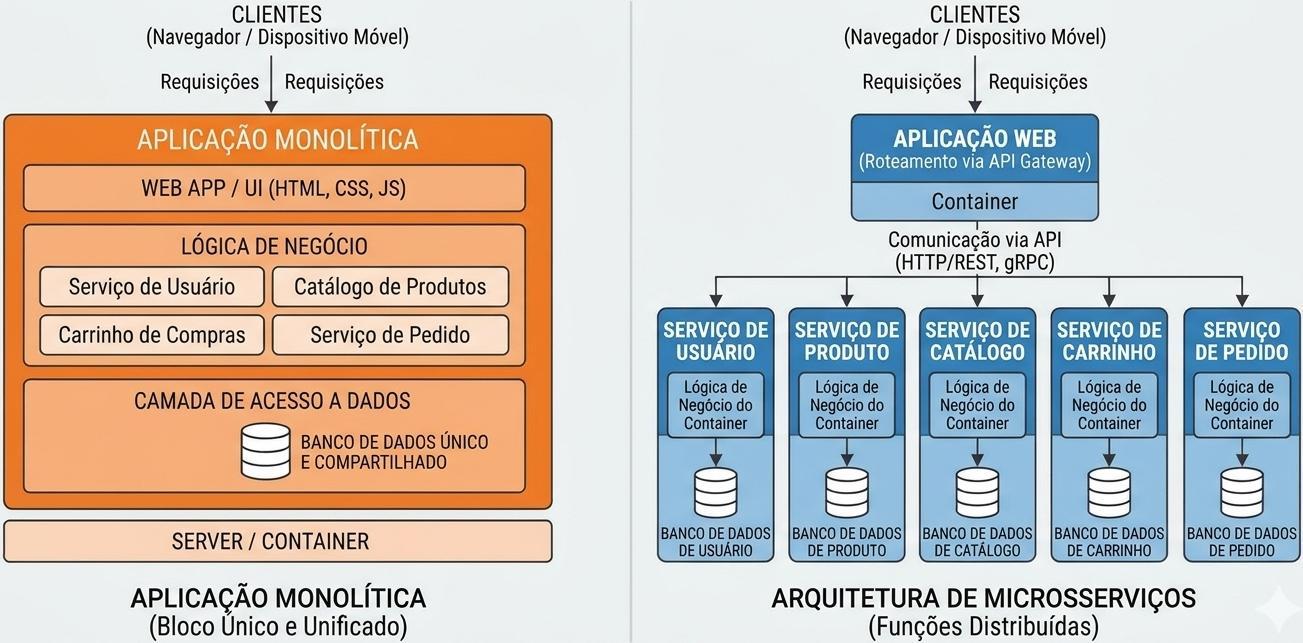
\includegraphics[width=1.0\linewidth]{figuras/monolitico_x_microservicos.jpg}
    \caption{Comparação entre a organização da funcionalidade de uma aplicação monolítica e uma com microserviços. Fonte: imagem gerada no Gemini a partir de prompt criado pelo autor.}
    \label{fig_mono_x_micro}
\end{figure}

%\subsection{Características Fundamentais} Não precisa quebrar em muitas subsseções

A transição para microsserviços se fundamenta em um conjunto de características e princípios arquiteturais estruturantes \cite{velepucha2023}. A primeira dessas características refere-se à componentização, que, conforme \citeonline{lewis2014}, significa a substituição da modularização local tradicional por serviços independentes expostos via rede. Essa mudança assegura que a substituição, atualização ou manutenção de um serviço específico ocorra sem a necessidade de recompactar ou reimplantar os demais componentes do ecossistema.

Outra diferença provocada pela substituição de módulos por serviços de rede é a presença de múltiplas tecnologias na construção da aplicação. Enquanto o monólito geralmente é construído com uma única linguagem e/ou um único \textit{framework} para toda a aplicação, os microsserviços viabilizam a adoção de diversas tecnologias, formando uma chamada "arquitetura poliglota" \cite{richardson2018}. Dessa forma, cada microsserviço é construído com a linguagem ou biblioteca que melhor se adapta à funcionalidade implementada.

Com relação ao gerenciamento da informação, o isolamento de dados por serviço é apontado como um pilar incontornável \cite{lewis2014}. Cada microsserviço deve possuir e gerenciar seu próprio repositório de dados privado, sendo impedido o acesso direto de serviços externos ao seu banco de dados. Qualquer interação ou consulta a informações sob domínio de outro serviço deve ocorrer exclusivamente por meio de sua API pública, eliminando o acoplamento no nível do banco de dados. Consequentemente, assim como ocorre no código da aplicação, existe também a possibilidade de adoção de uma persistência poliglota \cite{richardson2018}. Por exemplo, um serviço de catálogo de produtos pode adotar um banco NoSQL orientado a documentos para otimização de leitura, enquanto o serviço de carrinho de compras utiliza um banco chave-valor em memória para alta performance, e o serviço de pedidos utiliza um banco relacional garantidor de transações atômicas \cite{richardson2018}.

Por fim, a separação física entre processos contribui para uma maior robustez e o isolamento de falhas. Em uma arquitetura monolítica tradicional, uma exceção não tratada pode paralisar todo o processo computacional. Por outro lado, com microsserviços, a indisponibilidade pontual de um serviço específico não provoca o colapso de toda a aplicação, impedindo a propagação de falhas em cascata e permitindo que funcionalidades não afetadas continuem operando normalmente para o usuário final \cite{newman2021}.

%\subsection{Desafios da Arquitetura de Microsserviços}

Apesar dos benefícios de disponibilidade e desacoplamento, a adoção de microsserviços introduz uma série de complexidades típicas dos sistemas distribuídos \cite{lewis2014, soylemez2022}: (1) maior dependência dos serviços de rede; (2) a maior latência das requisições via rede; (3) maior complexidade devido ao emprego de diferentes tecnologias; e (4) maior dificuldade no diagnóstico de falhas.

Sobre esse último ponto, enquanto em um monólito a depuração ocorre pela análise de um log único e unificado, em microsserviços a execução de uma única requisição de usuário atravessa vários serviços independentes via rede \cite{richardson2018}. Essa pulverização de processos torna a identificação das causas de erros um desafio complexo. Para contornar essa dificuldade e correlacionar os registros de auditoria espalhados entre diversos \textit{containers}, torna-se indispensável a implementação de técnicas de rastreamento distribuído (\textit{distributed tracing}), injetando identificadores únicos de correlação em todas as chamadas de rede \cite{richardson2018}.

%Além disso, a substituição de transações locais por modelos de consistência eventual exige a reformulação do fluxo de dados. A coordenação de estados entre serviços passa a demandar padrões avançados, tais como a Arquitetura Baseada em Eventos e o Padrão Saga \cite{richardson2018}. Dessa forma, a transição para microsserviços representa uma escolha consciente (\textit{trade-off}): reduz-se a complexidade interna do código-fonte e ganha-se resiliência, em troca do aumento da complexidade de infraestrutura, rastreabilidade e comunicação de rede.

\section{Padrões de Decomposição}

Neste projeto serão utilizados três diferentes padrões de decomposição de aplicações monolíticas para microsserviços. Cada um deles é descrito nas seções seguintes.


\subsection{Decomposição por Capacidade de Negócio}
% Visão macro e processual.

A decomposição por capacidade de negócio (\textit{Decompose by Business Capability}) fundamenta-se na identificação das funções operacionais e processos que a organização executa para atingir seus objetivos \cite{richardson2018}. Nesse contexto, uma capacidade de negócio representa o objetivo funcional da organização (o que é realizado) em contraste com as tecnologias usadas no momento (como é realizado).

Dessa forma, a conceituação de uma capacidade permanece estável ao longo do tempo, independentemente das transformações nas ferramentas de software ou na infraestrutura. Por exemplo, a capacidade de "Gestão de Estoque" ou de "Processamento de Pedidos" representa uma necessidade operacional contínua de uma organização comercial, quer seja executada por meio de registros manuais, por um sistema monolítico legado ou por microsserviços isolados.

Nessa estratégia, as fronteiras dos microsserviços são alinhadas às áreas funcionais da organização. Em um sistema corporativo, por exemplo, funções como gestão de estoque, processamento de pedidos e faturamento dão origem a serviços independentes. A principal vantagem teórica dessa abordagem consiste no alinhamento direto entre a estrutura do software e a estrutura organizacional, o que favorece a atribuição de equipes autônomas responsáveis pelo ciclo de vida completo de cada serviço \cite{newman2021}.

Entretanto, essa abordagem apresenta limitações quando aplicada a sistemas monolíticos legados que utilizam um banco de dados relacional compartilhado. Como diferentes processos de negócio frequentemente acessam e alteram as mesmas tabelas, a divisão dos serviços baseada apenas na capacidade funcional pode exigir a implementação de transações distribuídas e gerar dependências cruzadas entre os novos serviços.



\subsection{Decomposição por Subdomínio (DDD)}
% Visão de fronteiras lógicas e isolamento de dados.

A decomposição por subdomínio baseia-se nos princípios do \textit{Domain-Driven Design} (DDD), propostos por \citeonline{evans2003} e aplicados à arquitetura de microsserviços por \citeonline{richardson2018}. Nessa abordagem, o domínio do sistema é particionado em subdomínios, classificados em centrais, de suporte e genéricos, sendo cada um associado a um Contexto Delimitado (\textit{Bounded Context}).

O conceito de \textit{Bounded Context} estabelece que cada modelo de dados e vocabulário técnico possui significado estrito dentro de seus limites lógicos \cite{evans2003}. Por exemplo, a entidade "Cliente" no contexto de vendas possui atributos e regras de negócio distintos da mesma entidade no contexto de atendimento ou faturamento.

No contexto experimental deste trabalho, a decomposição por subdomínio orienta a separação física dos serviços com base no isolamento dos modelos de dados. Essa estratégia busca reduzir o acoplamento conceitual e assegurar que cada microsserviço mantenha a consistência de seu modelo dentro de um repositório de dados privado, eliminando o acesso direto a bancos de dados compartilhados \cite{newman2020}.


\subsection{Decomposição por Transações}
% Visão de consistência técnica (ACID).

A decomposição por transações (\textit{Decompose by Transactions}) adota um critério técnico focado na consistência dos dados para a definição das fronteiras dos microsserviços \cite{richardson2018}. Diferente das abordagens orientadas a processos ou domínios de negócio, essa estratégia prioriza a análise das restrições ACID (\textit{Atomicity, Consistency, Isolation, Durability}) e do fluxo de operações de escrita no banco de dados.

Na refatoração de uma aplicação monolítica, a divisão de um banco de dados relacional centralizado pode transformar transações locais em transações distribuídas entre diferentes serviços. A coordenação dessas transações via rede adiciona complexidade e reduz a vazão do sistema \cite{richardson2018}. Para evitar a degradação de desempenho e a complexidade operacional, a decomposição por transações agrupa no mesmo microsserviço os módulos e tabelas que exigem escrita atômica e consistência imediata. Operações que suportam consistência eventual são isoladas em serviços assíncronos. Na matriz experimental desta pesquisa, essa abordagem atua como contraponto técnico voltado à redução de chamadas de rede e à preservação da integridade transacional \cite{newman2021}.

\section{Métricas e Instrumentos de Coleta}
\label{sec:metricas_coleta}
% Apresentar as ferramentas (Docker stats, GitHub Actions, Autocannon, Madge/ESLint).

Neste projeto, para avaliar os três padrões de decomposição citados, serão adotadas um conjunto de métricas, cuja descrição de cada uma é apresentada nesta seção.


\subsection{Métricas de Agilidade e DevOps}

Para avaliar o impacto da decomposição na operabilidade e no ciclo de vida do software, esta dimensão foca na agilidade de entrega e na inicialização dos serviços:
\begin{itemize}
    \item \textbf{Tempo de Construção:} Mensura a duração total dos processos de empacotamento e geração das imagens Docker para cada microsserviço ou snapshot, avaliando a granularidade do pipeline de CI/CD.
    \item \textbf{Tempo de Inicialização:} Registra o intervalo necessário desde o comando de execução até a prontidão completa do serviço para receber requisições de rede (prontidão de escuta nas portas configuradas).
\end{itemize}

\subsection{Métricas de Custo Operacional e Infraestrutura}
\label{sec:metricas_infraestrutura}

O consumo de recursos computacionais é monitorado de forma isolada por contêiner para mensurar o \textit{overhead} introduzido pela distribuição da arquitetura:
\begin{itemize}
    \item \textbf{Uso de CPU e Memória:} Coletados por meio de ferramentas de monitoramento de contêineres, registrando a média e o pico de consumo de processamento e RAM durante a execução sob carga.
    \item \textbf{Uso de Armazenamento:} Avalia o impacto do particionamento e da duplicação de dependências analisando o tamanho final das imagens Docker geradas para cada componente da arquitetura.
\end{itemize}

\subsection{Métricas de Desempenho}
% Latência de API e Vazão Máxima.

Para avaliar o comportamento dinâmico e o impacto de gargalos operacionais gerados pela transição arquitetural, a pesquisa emprega métricas de desempenho, com ênfase na latência de API e na vazão máxima (\textit{throughput}). O fundamento empírico dessas medições baseia-se na identificação de restrições de desempenho provocadas pela conversão de dependências locais em chamadas de rede. Conforme apontam \citeonline{richardson2018} e \citeonline{newman2020}, a introdução da comunicação interprocessos (IPC) nas fronteiras dos microsserviços adiciona sobrecarga temporal que afeta diretamente a eficiência do sistema.

A latência é quantificada por meio de percentis, que revelam o comportamento sob estresse e a estabilidade nos tempos de resposta da aplicação. Ademais, a vazão máxima mensura o volume limite de requisições processadas por segundo sob condições controladas de concorrência. Nesse sentido, essas métricas permitem correlacionar diretamente a eficiência operacional da aplicação com o grau de acoplamento distribuído e a sobrecarga de rede imposta por cada abordagem de decomposição.



\subsection{Métricas de Manutenibilidade e Complexidade}
\label{sec:metricas_manutenibilidade}

Para avaliar a evolução estrutural da arquitetura ao longo da refatoração, a pesquisa emprega métricas voltadas à manutenibilidade e complexidade, com destaque para as Linhas de Código (LOC), a contagem de componentes físicos e o cruzamento de fronteiras. O fundamento teórico para a análise desse acoplamento baseia-se no conceito de conascência (\textit{connascence}), definido formalmente como a interdependência na qual a alteração em um elemento de software exige a modificação de outro para preservar a corretude do sistema \cite{pagejones1992}. O objetivo central do \textit{design} de arquiteturas modulares é a minimização da conascência e do cruzamento de fronteiras entre domínios distintos.

No monólito, o cruzamento de fronteiras é observado como conascências estáticas de nome e tipo, quantificadas por meio de análise estática do código-fonte. Durante a transição para microsserviços por meio do padrão \textit{Strangler Fig}, a remoção dessas dependências físicas evita o acoplamento indesejado que, conforme alertam \citeonline{newman2020} e \citeonline{richardson2018}, converte simples chamadas locais de código em comunicações síncronas via rede (\textit{Inter-Process Communication} - IPC). Além disso, o rastreamento das Linhas de Código (LOC) e do número de componentes físicos permite mensurar o esforço de refatoração, o dimensionamento dos artefatos e o impacto do isolamento em cada estágio da pesquisa.

\section{Engenharia de Software Experimental}
\label{sec:eng_software_experimental}

A condução de pesquisas empíricas na área de computação exige o rigor metodológico característico da Engenharia de Software Experimental \cite{wohlin2012}. Conforme discutem \citeonline{kitchenham2002}, abordagens experimentais permitem avaliar tecnologias, métodos e ferramentas de software em ambientes controlados, fornecendo evidências quantitativas sobre os seus reais impactos, benefícios e limitações.

No contexto de refatoração arquitetural, a experimentação controlada por meio de matrizes comparativas e métricas reprodutíveis, como análise estática de código e testes de carga dinâmicos, é fundamental para mitigar vieses subjetivos. Isso possibilita que decisões de migração de monólitos para microsserviços sejam sustentadas por dados empíricos sólidos e mensuráveis.

\section{Ferramentas}

Pequeno paragrafo

\subsection*{Docker}
A plataforma de conteinerização \textit{Docker} foi adotada para garantir o isolamento consistente dos ambientes de execução em todas as fases da pesquisa. Além de prover portabilidade e padronizar o empacotamento dos serviços, o ambiente conteinerizado viabiliza a coleta controlada de métricas de infraestrutura, permitindo extrair o consumo computacional de CPU e o uso de memória RAM por meio do comando \textit{docker stats} durante os testes experimentais.

\subsection*{Madge}
O \textit{Madge} é uma ferramenta de análise estática de código-fonte utilizada para rastrear, analisar e visualizar grafos de dependência em projetos desenvolvidos em JavaScript e TypeScript. No escopo deste trabalho, o \textit{Madge} é empregado para quantificar o acoplamento estático e o cruzamento de fronteiras (\textit{cross-domain calls}), permitindo auditar o número de importações interdomínio que configuram a conascência de código no monólito base e nas etapas de refatoração.

\subsection*{Autocannon}
O \textit{Autocannon} é uma ferramenta de teste de carga e estresse de alta performance voltada para aplicações HTTP em Node.js. Na matriz experimental desta pesquisa, o \textit{Autocannon} atua como o motor de estresse dinâmico para avaliar o desempenho das APIs em cada \textit{snapshot} arquitetural, permitindo mensurar métricas críticas como a latência de resposta e a vazão máxima de requisições por segundo sob condições controladas de concorrência.

\subsection*{NGINX}
O \textit{NGINX} é um servidor web e proxy reverso de alta performance, projetado para lidar com alto volume de conexões simultâneas com baixo consumo de memória. No escopo desta pesquisa, o \textit{NGINX} atua como o mecanismo operacional do padrão \textit{Strangler Fig}, posicionado na borda da arquitetura para interceptar e redistribuir o tráfego de rede entre a aplicação monolítica e os microsserviços extraídos. Por meio de regras de roteamento baseadas em prefixos de rotas (URIs), o proxy permite direcionar chamadas para os novos contêineres sem exigir modificações nos clientes consumidores.


\chapter{Trabalhos Relacionados}

Nesta seção, são analisados estudos anteriores que investigaram abordagens de decomposição de aplicações monolíticas, técnicas de identificação de microsserviços e avaliações comparativas de estratégias de migração de arquitetura. Cada trabalho é apresentado com seu objetivo, a técnica empregada e os resultados alcançados, seguido de uma discussão sobre como este trabalho se posiciona em relação às lacunas identificadas. 

\textcite{levcovitz2016} propõem uma técnica para extração de microsserviços a partir de sistemas corporativos monolíticos de grande porte, validada sobre um sistema bancário legado de aproximadamente 750 mil linhas de código. A técnica analisa o esquema relacional do banco de dados, identificando agrupamentos de tabelas fortemente conectadas por chaves estrangeiras e por transações que operam em conjunto, sem exigir a reescrita do código-fonte da aplicação original. Como resultado, os autores demonstram que é possível identificar automaticamente candidatos a microsserviços coerentes com domínios de negócio reais a partir apenas da estrutura de dados, validando a viabilidade de uma decomposição orientada a transações mesmo em sistemas legados de grande escala.

\textcite{kazanavicius2020} comparam a decomposição de uma mesma aplicação corporativa legada utilizando diferentes métodos de identificação de microsserviços. A metodologia consiste em aplicar múltiplas heurísticas de particionamento ao mesmo sistema e definir critérios de avaliação para julgar as vantagens e desvantagens de cada resultado obtido. Os autores concluem que metodologias distintas produzem particionamentos significativamente diferentes do mesmo sistema, cada um com trade-offs próprios, e propõem um conjunto de critérios qualitativos para orientar a escolha da estratégia mais adequada a um determinado contexto.

\textcite{wang2024} comparam, de forma independente, oito ferramentas automáticas de decomposição de microsserviços. Os autores aplicam essas ferramentas a quatro aplicações monolíticas selecionadas sistematicamente: três delas já haviam sido utilizadas em pesquisas anteriores sobre decomposição, e uma quarta aplicação foi incluída propositalmente por nunca ter sido decomposta antes, para testar a generalização das ferramentas. Combinando métricas quantitativas de modularidade e de similaridade estrutural com entrevistas junto a desenvolvedores responsáveis por duas das aplicações, os autores constatam que nenhuma ferramenta se destaca de forma consistente em todos os cenários avaliados, ou seja, o desempenho de cada uma depende de características específicas da aplicação analisada. Além disso, destacam que nenhuma das ferramentas avaliadas produz uma decomposição efetivamente executável.

\textcite{barzotto2022} investigam, por meio de um estudo de caso empírico na indústria financeira, os impactos da decomposição de um módulo crítico (saque em dinheiro em terminais de autoatendimento) de uma aplicação monolítica em Java/Spring para uma arquitetura baseada em microsserviços. Os autores compararam a versão monolítica com a versão decomposta utilizando métricas clássicas de modularidade de código orientado a objetos e testes de estresse de carga via Gatling para medir o consumo de hardware. Os resultados apontaram ganhos de modularidade e redução no consumo computacional após a decomposição. Entretanto, os autores reportaram limitações técnicas na medição de hardware do sistema monolítico legado e avaliaram apenas uma única aplicação com um método de decomposição direcionado por DDD.


\begin{table}[htbp]
\caption{Comparação dos trabalhos relacionados}
\label{tab:trabalhos_relacionados}
\centering
\small
\renewcommand{\arraystretch}{1.15}
\begin{tabularx}{\textwidth}{@{}>{\raggedright\arraybackslash}p{2.4cm} >{\raggedright\arraybackslash}X >{\raggedright\arraybackslash}X >{\raggedright\arraybackslash}X >{\raggedright\arraybackslash}X@{}}
\hline
\textbf{Trabalho} & \textbf{Objetivo} & \textbf{Técnica} & \textbf{Resultado principal} & \textbf{Lacuna em relação a este trabalho} \\
\hline
 
Levcovitz, Terra e Valente (2016) &
Extrair microsserviços de um monólito &
Análise do esquema relacional &
Agrupou tabelas coerentes em 1 sistema bancário &
1 sistema; sem migração real; sem métricas dinâmicas \\
\hline
 
Kazanavičius e Mažeika (2020) &
Comparar metodologias no mesmo sistema &
Heurísticas de particionamento + critérios qualitativos &
Metodologias distintas geram partições distintas &
1 sistema; avaliação qualitativa \\
\hline
 
Wang, Bornais e Rubin (2024) &
Comparar ferramentas automáticas &
8 ferramentas em 4 benchmarks + entrevistas &
Nenhuma ferramenta domina; depende da aplicação &
Ferramentas automáticas, não metodologias manuais \\
\hline

Barzotto e Farias (2022) &
Avaliar impactos de decomposição na indústria &
Estudo de caso (Java/Spring) + métricas CK + Gatling &
Microsserviços apresentaram maior modularidade e menor consumo de recursos &
1 sistema; 1 metodologia; medições incompletas no monólito \\
\hline
 
\textbf{Este trabalho} &
Comparar 3 metodologias em 3 sistemas &
Estudo empírico comparativo ($3 \times 3$) + Strangler Fig + métricas estáticas e dinâmicas &
\textit{(Cap. 5)} &
--- \\
\hline
\end{tabularx}
\legend{Fonte: Elaborado pelo autor.}
\end{table}


A Tabela \ref{tab:trabalhos_relacionados} destaca as principais diferenças entre os trabalhos relacionados e esta pesquisa. Os estudos relacionados revelam lacunas centrais que este trabalho busca explorar. Primeiramente, \textcite{wang2024} mostram que o desempenho das técnicas de decomposição depende fortemente de características específicas de cada aplicação, o que limita a generalização de conclusões obtidas sobre um conjunto restrito de benchmarks tradicionais. Este trabalho utiliza três aplicações de código aberto desenvolvidas de forma independente, com arquitetura e complexidade que representam sistemas reais. Além disso, enquanto \textcite{kazanavicius2020} e \textcite{barzotto2022} limitam suas investigações empíricas a uma única aplicação e a abordagens isoladas de decomposição, este trabalho estabelece um estudo empírico comparativo avaliando sistematicamente três metodologias de decomposição sobre três sistemas de contextos diferentes. Por fim, ao contrário de abordagens com foco analítico como a de \textcite{levcovitz2016}, este trabalho executa e instrumenta as migrações incrementais mediadas pelo padrão \textit{Strangler Fig}, combinando métricas estáticas de modularidade com ensaios dinâmicos de desempenho e observabilidade de infraestrutura conteinerizada ao longo de múltiplos marcos de transição (\textit{snapshots}).

\chapter{Metodologia}
\label{cap:metodologia}

% Introdução breve do capítulo explicando que a pesquisa tem caráter empírico e quantitativo, 
% focando na comparação de três padrões de decomposição em três aplicações distintas.

Este capítulo descreve a metodologia de pesquisa adotada para conduzir este estudo empírico comparativo sobre estratégias de decomposição de monólitos em microsserviços. A pesquisa é baseada na Engenharia de Software Experimental, estruturando-se a partir da refatoração de três aplicações monolíticas de código aberto, submetidas a três metodologias distintas de decomposição arquitetural.

A metodologia foi desenhada para que seja possível coletar e analisar dados de experimentos quantitativos ao longo do processo de migração, utilizando o padrão \textit{Strangler Fig} como mecanismo para a extração incremental. A observação dos experimentos ocorre de forma iterativa por meio de marcos de transição (\textit{snapshots}), o que permite avaliar o impacto de cada estratégia em quatro categorias: agilidade, infraestrutura, desempenho e manutenibilidade.

As seções a seguir detalham o desenho do experimento do estudo comparativo, a caracterização e seleção dos estudos de caso, os critérios de decomposição, os procedimentos operacionais de transição por \textit{snapshots} e os instrumentos de coleta de dados.

\section{Desenho da Pesquisa e Abordagem Experimental}
\label{sec:desenho_pesquisa}

A pesquisa é orientada pelo paradigma da Engenharia de Software Experimental, adotando uma estrutura $3 \times 3$ que cruza três objetos de estudo distintos com três tratamentos arquiteturais independentes. Essa divisão permite avaliar se os efeitos decorrentes de cada estratégia de decomposição são consistentes entre domínios diferentes de aplicação ou se dependem fortemente das características próprias do sistema sob refatoração.

O experimento fundamenta-se na definição explícita de variáveis independentes e dependentes:
\begin{itemize}
    \item \textbf{Variáveis Independentes:}
    \begin{enumerate}
        \item{Metodologia de Decomposição Arquitetural:} Decomposição por Capacidade de Negócio, Decomposição por Subdomínio e Decomposição por Transações.
        \item{Domínio e Características da Aplicação:} Sistema de Inventário, Sistema de Leilões e Sistema de E-commerce.
    \end{enumerate}
    \item \textbf{Variáveis Dependentes:} O impacto de cada abordagem é medido por meio das quatro categorias de medição definidas na Seção \ref{sec:metricas_coleta}:
    \begin{enumerate}
        \item{Agilidade:} Tempo de compilação e construção de imagens Docker e tempo de inicialização dos serviços;
        \item{Infraestrutura:} Consumo de processamento (CPU), consumo de memória RAM e volume de armazenamento;
        \item{Desempenho:} Vazão máxima de requisições por segundo e percentis de latência de resposta ($p_{50}$, $p_{90}$, $p_{99}$);
        \item{Manutenibilidade:} Linhas de Código (LOC), contagem de componentes físicos e violações de fronteiras lógicas.
    \end{enumerate}
\end{itemize}

A metodologia prevê a execução de nove trilhas de refatoração independentes, partindo do mesmo ponto para cada aplicação. Cada trilha é submetida a testes padronizados de estresse e avaliação estática de código a cada tranformação.

\section{Seleção e Justificativa das Aplicações}
\label{sec:selecao_aplicacoes}

Para assegurar a validade e a relevância prática dos resultados, evitou-se o uso de sistemas de teste artificiais. Com base nisso, foram selecionadas três aplicações monolíticas de código aberto desenvolvidas em TypeScript com o ecossistema NestJS, que representam propostas e requisitos não funcionais diferentes encontrados na indústria de software.

\begin{itemize}
    \item \textbf{Aplicação Crítica: Sistema de Inventário.} A aplicação \textit{inventory-api}\footnote{Disponível em: \url{https://github.com/egp1020/inventory-api}.} representa um sistema de controle de inventário e execução operacional, similar aos sistemas MES (\textit{Manufacturing Execution System}) industriais. Nesse contexto, é uma aplicação que demanda acesso em tempo real, de modo a não tolerar tempos elevados fora do ar. Além disso, a integridade das transações nos bancos de dados é fundamental: transações operacionais de baixa e transferência de materiais exigem atualizações imediatas entre armazéns, produtos e saldos em estoque, sendo inadmissível o registro de quantidades negativas.
    
    \item \textbf{Aplicação de Alta Concorrência: Monitor de Mercado e Leilões.} A aplicação \textit{auction}\footnote{Disponível em: \url{https://github.com/schoibs/auction}.} representa o comportamento de plataformas de alta performance voltadas a leilões de cartas colecionáveis e negociação de ativos em tempo real. Esse contexto apresenta elevada concorrência de requisições síncronas de lances (\textit{bids}), atualização de preços em milissegundos e dispersão de eventos para múltiplos clientes conectados via WebSockets.
    
    \item \textbf{Aplicação Transacional e Catálogo: E-commerce.} A aplicação \textit{ecommerce}\footnote{Disponível em: \url{https://github.com/sappChak/nestjs-ecommerce}.} simboliza o varejo digital clássico, em que o volume de leitura supera em muito o de escrita, e cada carga exige uma estratégia própria. Por um lado, o catálogo de produtos exige alta vazão de leitura com dados desnormalizados, enquanto o carrinho e a finalização de pedidos precisam coordenar reservas, calcular taxas e acionar serviços auxiliares.
\end{itemize}

\section{Procedimentos de Migração e Marcos de Avaliação}
\label{sec:procedimentos_snapshots}

A condução das refatorações segue uma abordagem de evolução controlada, reduzindo interrupções no funcionamento global do sistema e permitindo aferir os impactos parciais de cada etapa de extração.

A transição da arquitetura de cada monólito para microsserviços é mediada pelo padrão \textit{Strangler Fig} \cite{fowler2004}, suportado por um proxy reverso configurado com o software NGINX.

O proxy atua como um ponto único de entrada de tráfego de rede para a aplicação. Nos estágios iniciais, as requisições são encaminhadas diretamente ao monólito. Conforme módulos específicos são extraídos para microsserviços independentes, as regras de roteamento baseadas em prefixos de caminhos são reconfigurados dinamicamente no proxy. O tráfego direcionado aos módulos refatorados passa a ser interceptado e direcionado para os novos contêineres, sem que o monólito precise ser completamente desativado ou reescrito totalmente.

Para permitir que as mudanças e impactos sejam avaliados e rastreáveis, cada uma das 9 trilhas é dividida em quatro estados temporais, denominados \textit{snapshots}:

\begin{enumerate}
    \item \textbf{Snapshot 0 (Baseline Monolítico):} Corresponde ao código original da aplicação monolítica em execução, sem qualquer intervenção de arquitetura na base de serviços. Serve como linha de base para todas as métricas quantitativas;
    
    \item \textbf{Snapshot 1 (Primeira Extração Incremental):} Representa a extração inicial de um módulo funcional selecionado segundo as diretrizes de cada metodologia (tipicamente um serviço de menor acoplamento ou de suporte), operando de forma desacoplada atrás do proxy reverso;
    
    \item \textbf{Snapshot 2 (Segunda Extração Incremental):} Representa a evolução da migração com a separação de um segundo domínio ou capacidade operacional, ampliando as fronteiras de rede e a comunicação interserviços;
    
    \item \textbf{Snapshot Final (Decomposição Concluída):} Estado final em que todos os módulos previstos pela respectiva metodologia foram desacoplados em microsserviços independentes com persistência individual, desativando os componentes migrados do monólito.
\end{enumerate}

Cada marco de transição é feito por meio de tags no repositório de versionamento de código e submetido aos mesmos cenários de estresse de carga e amostragem de dados, para que as informações de desempenho, custo e acoplamento possam ser avaliadas conforme a evolução da arquitetura.


\chapter{Desenvolvimento}
\label{cap:desenvolvimento}

Este capítulo evidencia o desenvolvimento da pesquisa experimental. Nesse sentido, aqui está descrito em detalhes como cada aplicação era implementada, como se deu a aplicação das metodologias de decomposição e também os resultados, organizados em quadros para comparação.

\section{Arquitetura de Referência}
\label{sec:arquitetura_referencia}
Nessa seção, é apresentada a arquitetura base dos sistemas utilizadas na pesquisa. Com base nisso, avaliam-se os módulos, fronteiras e interações entre as partes de cada sistema, de modo que seja possível identificar como aplicar cada uma das metodologias sem impedir o funcionamento e o fluxo dos sistemas.

A padronização na linguagem TypeScript e na plataforma Node.js/NestJS assegura consistência nas comparações de Linhas de Código (LOC), no empacotamento em contêineres e permite uma comparação justa entre os tempos de inicialização e os perfis de consumo de recursos.

\subsection*{Sistema de Inventário}

O sistema de inventário foi desenvolvido como um monólito modular em NestJS, seguindo os princípios de Arquitetura Hexagonal e \textit{Domain-Driven Design}. A aplicação é organizada em quatro camadas por contexto: interface, aplicação, domínio e infraestrutura. Os seis contextos delimitados são autenticação, usuários, armazéns, produtos, movimentações e relatórios. Cada contexto possui seus próprios controladores REST, casos de uso, entidades e adaptadores de persistência.

O módulo compartilhado concentra as preocupações da base da aplicação, como autenticação e autorização, tratamento de exceções e acesso a dados. A persistência apoia-se em um único banco relacional, acessado por um mapeador objeto-relacional, e as operações que alteram o estoque exigem garantias transacionais.

A Figura \ref{fig:inventario_arquitetura} demonstra a arquitetura base do sistema.

\begin{figure}[h]
    \centering
    \caption{Arquitetura base do sistema de inventário.}
    \label{fig:inventario_arquitetura}
    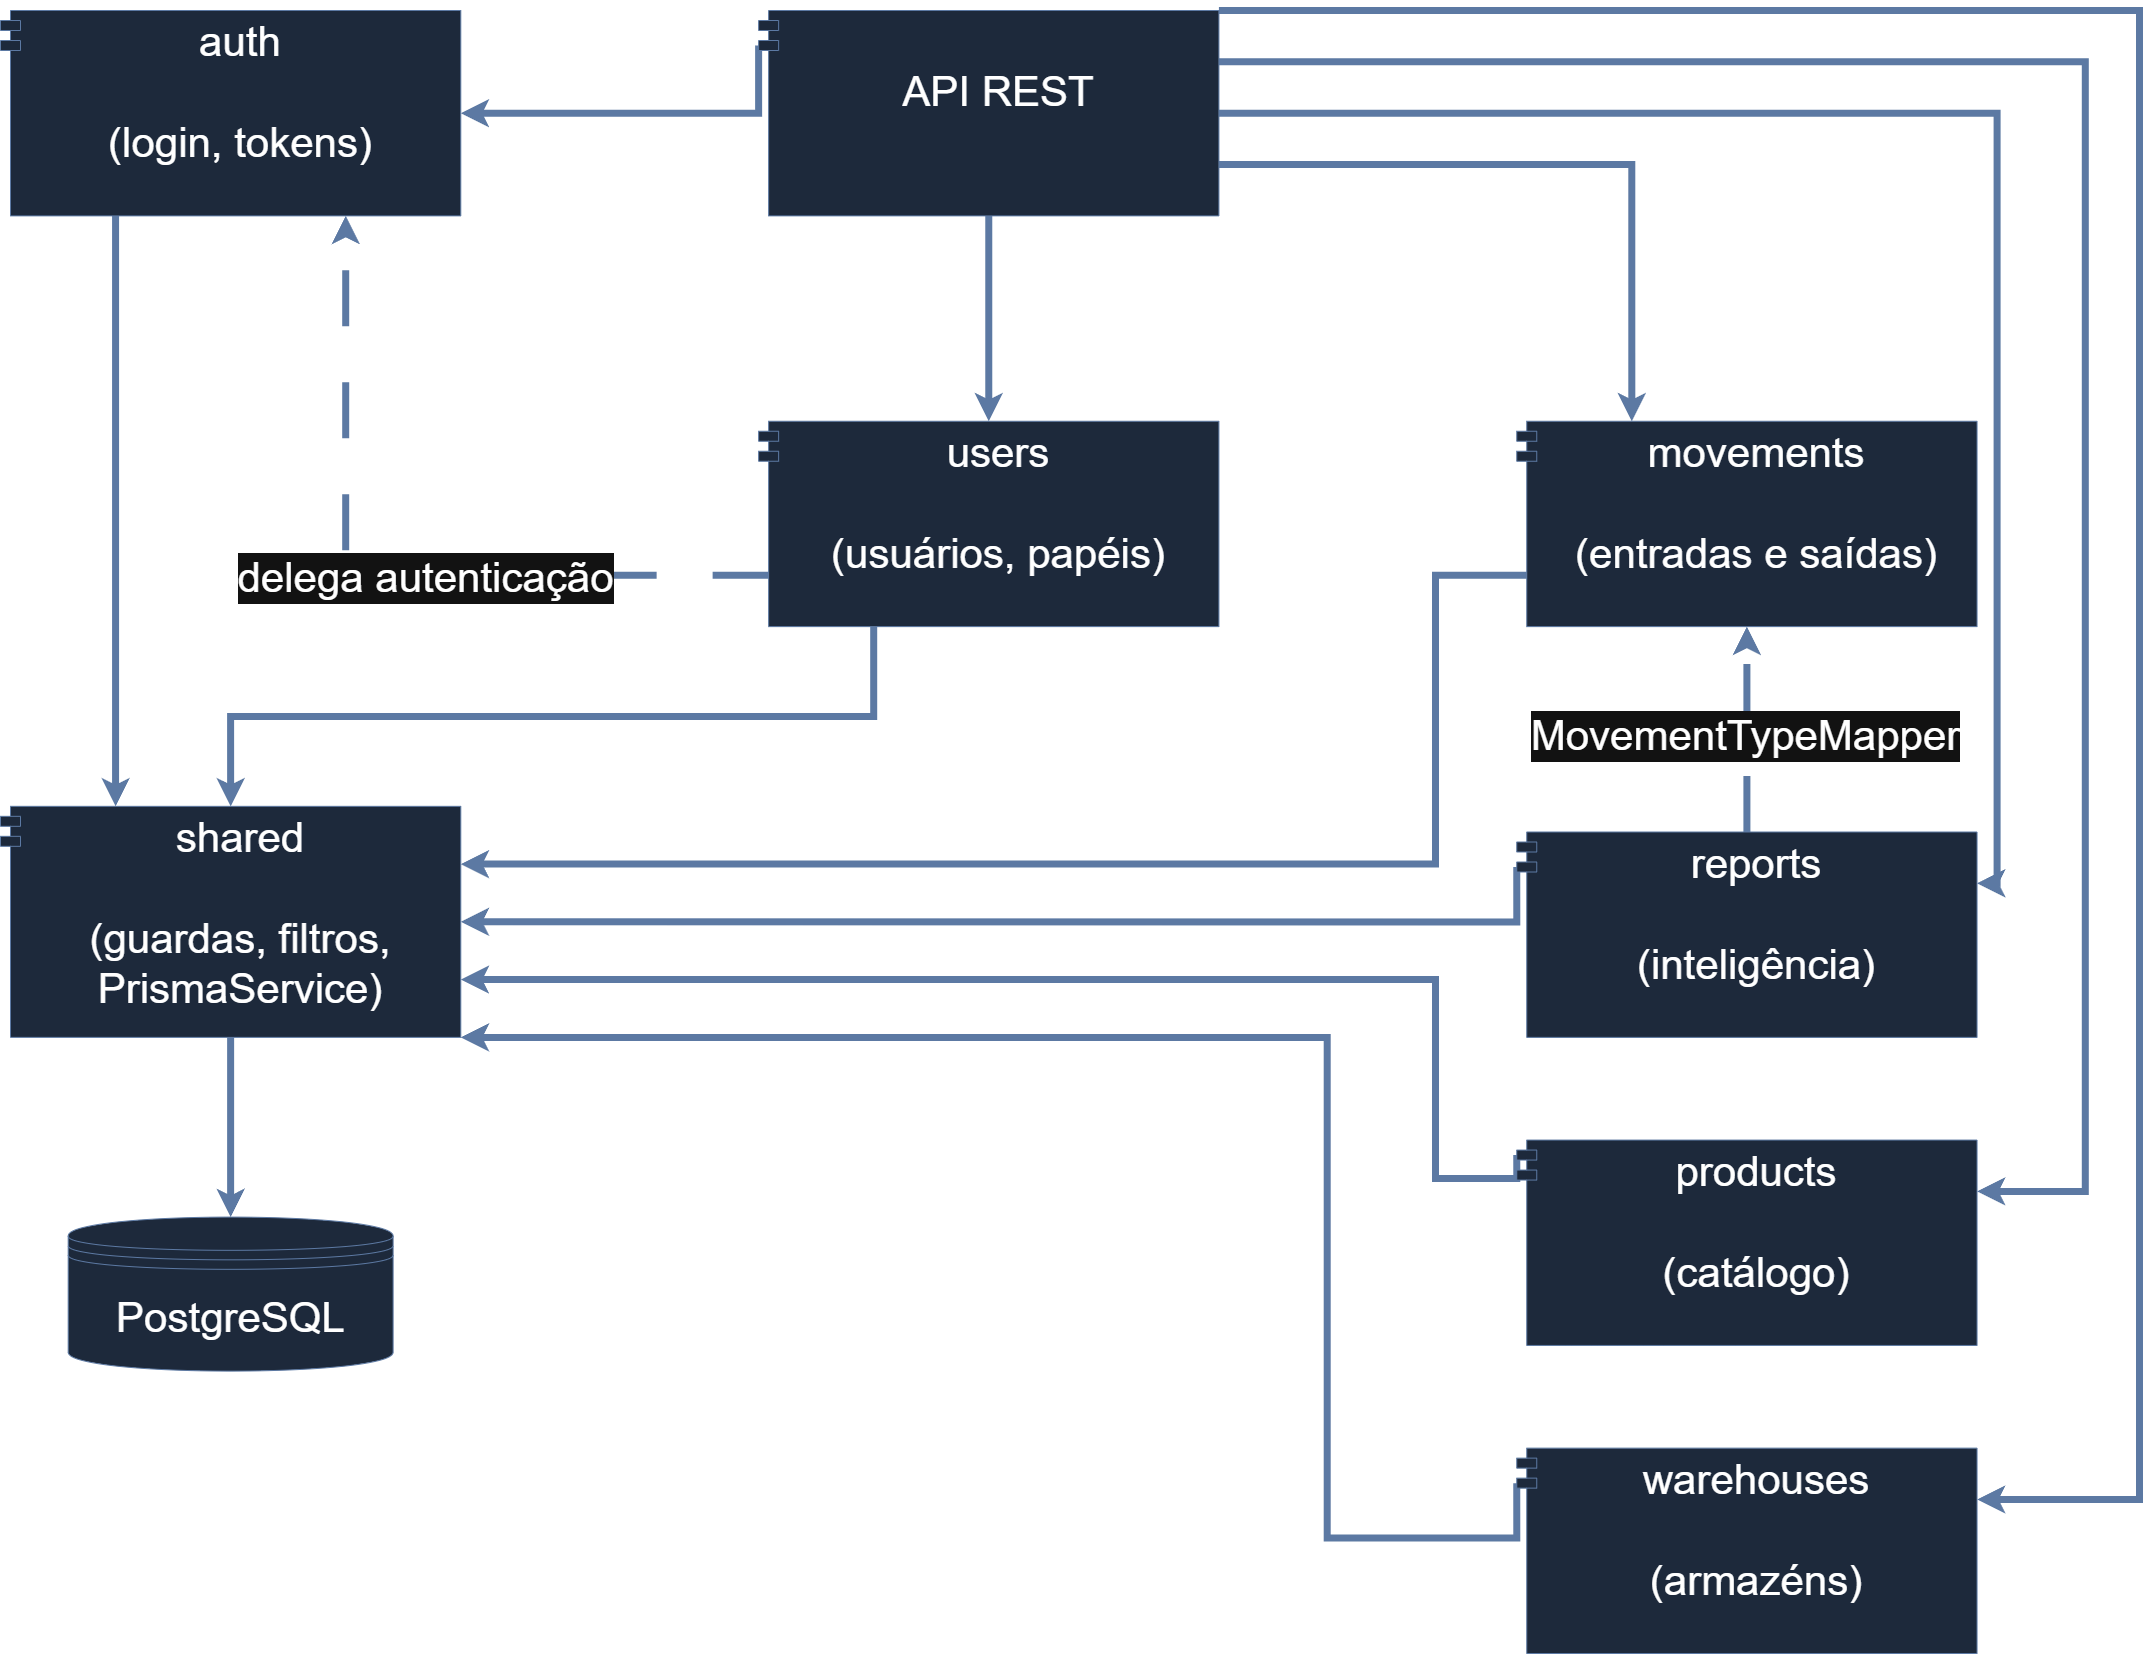
\includegraphics[width=0.7\textwidth]{figuras/inventario__arquitetura.png}
    \legend{Elaborado pelo autor (2026).}
\end{figure}

O Quadro \ref{qua:metricas-inventario-s0} reúne as métricas do sistema de inventário no estado inicial Snapshot 0, adotado como referência para o cálculo das variações das três metodologias de decomposição.

%% Fonte: metricas/inventory-api/capacidade-negocio/snapshot-0/tabelas/metricas.tex
\begin{quadro}[htb]
  \centering
  \caption{Métricas do sistema de inventário no baseline (Snapshot 0).}
  \label{qua:metricas-inventario-s0}
  \renewcommand{\arraystretch}{1.15}
  \begin{tabular}{|l|r|}
    \hline
    \textbf{Métrica} & \textbf{Valor} \\ \hline
    \multicolumn{2}{|l|}{\textbf{Agilidade e DevOps}} \\ \hline
    Tempo de construção (média) & 46.746 ms \\
    Tempo de inicialização (média) & 9.155 ms \\ \hline
    \multicolumn{2}{|l|}{\textbf{Custo e Infraestrutura}} \\ \hline
    CPU total (repouso / carga) & 2,22 \% / 241,0 \% \\
    RAM total (repouso / carga) & 86,3 MB / 188,5 MB \\
    Imagem da aplicação & 151,6 MB \\ \hline
    \multicolumn{2}{|l|}{\textbf{Desempenho}} \\ \hline
    \texttt{products} --- vazão & 557,2 req/s \\
    \texttt{products} --- latência p50/p90/p99 & 34,7 / 38,7 / 45,0 ms \\
    \texttt{reports/movements} --- vazão & 350,8 req/s \\
    \texttt{reports/movements} --- latência p50/p90/p99 & 55,0 / 61,0 / 105,3 ms \\
    \texttt{reports/stock} --- vazão & 201,3 req/s \\
    \texttt{reports/stock} --- latência p50/p90/p99 & 97,7 / 103,3 / 114,0 ms \\
    \texttt{movements} --- vazão & 311,9 req/s \\
    \texttt{movements} --- latência p50/p90/p99 & 63,0 / 72,3 / 89,0 ms \\ \hline
    \multicolumn{2}{|l|}{\textbf{Manutenibilidade}} \\ \hline
    Linhas de Código & 8.783 \\
    Componentes / contêineres & 2 / 2 \\
    Chamadas entre fronteiras & 69 de 389 \\ \hline
  \end{tabular}
  \fonte{medição automatizada do experimento (média de três execuções).}
\end{quadro}


\subsection*{Sistema de Leilões}

O monólito utiliza o ORM TypeORM conectado ao PostgreSQL, auxiliado pelo Redis para controle de filas e processamento de tarefas em segundo plano via BullMQ e transmissão de mensagens em tempo real. Múltiplos componentes com ciclo de vida assíncrono e de operações transacionais críticas de encerramento de lance e transferência de ativos permite observar a latência sob estresse e a vazão de requisições durante a transição dos serviços.

\subsection*{E-commerce}

Desenvolvida sobre o NestJS com o ODM Mongoose conectado a um banco de dados orientado a documentos (MongoDB), o código fonte original se organizava em mais de 20 controladores que cobriam autenticação, produtos, carrinho, pedidos, estoque e avaliações. Por conta desse volume, a fim de focar a experimentação na regra de negócio principal, foi necessário reduzir a complexidade do sistema ao cortar módulos que se integravam com ferramentas de terceiros, como AWS para armazenamento em núvem e Stripe para pagamentos, que se transformaram em módulos locais. Além disso, alguns componentes que complementavam o sistema, como aluguel, ofertas de serviços e chat também foram removidos. Desta forma, sua estrutura final permite investigar os impactos da decomposição em modelos orientados a documentos e em como o pedido grava status e estoque das operações de finalização de compras.

A Figura \ref{fig:ecommerce_arquitetura} demonstra a arquitetura base do sistema.


\begin{figure}
    \centering
    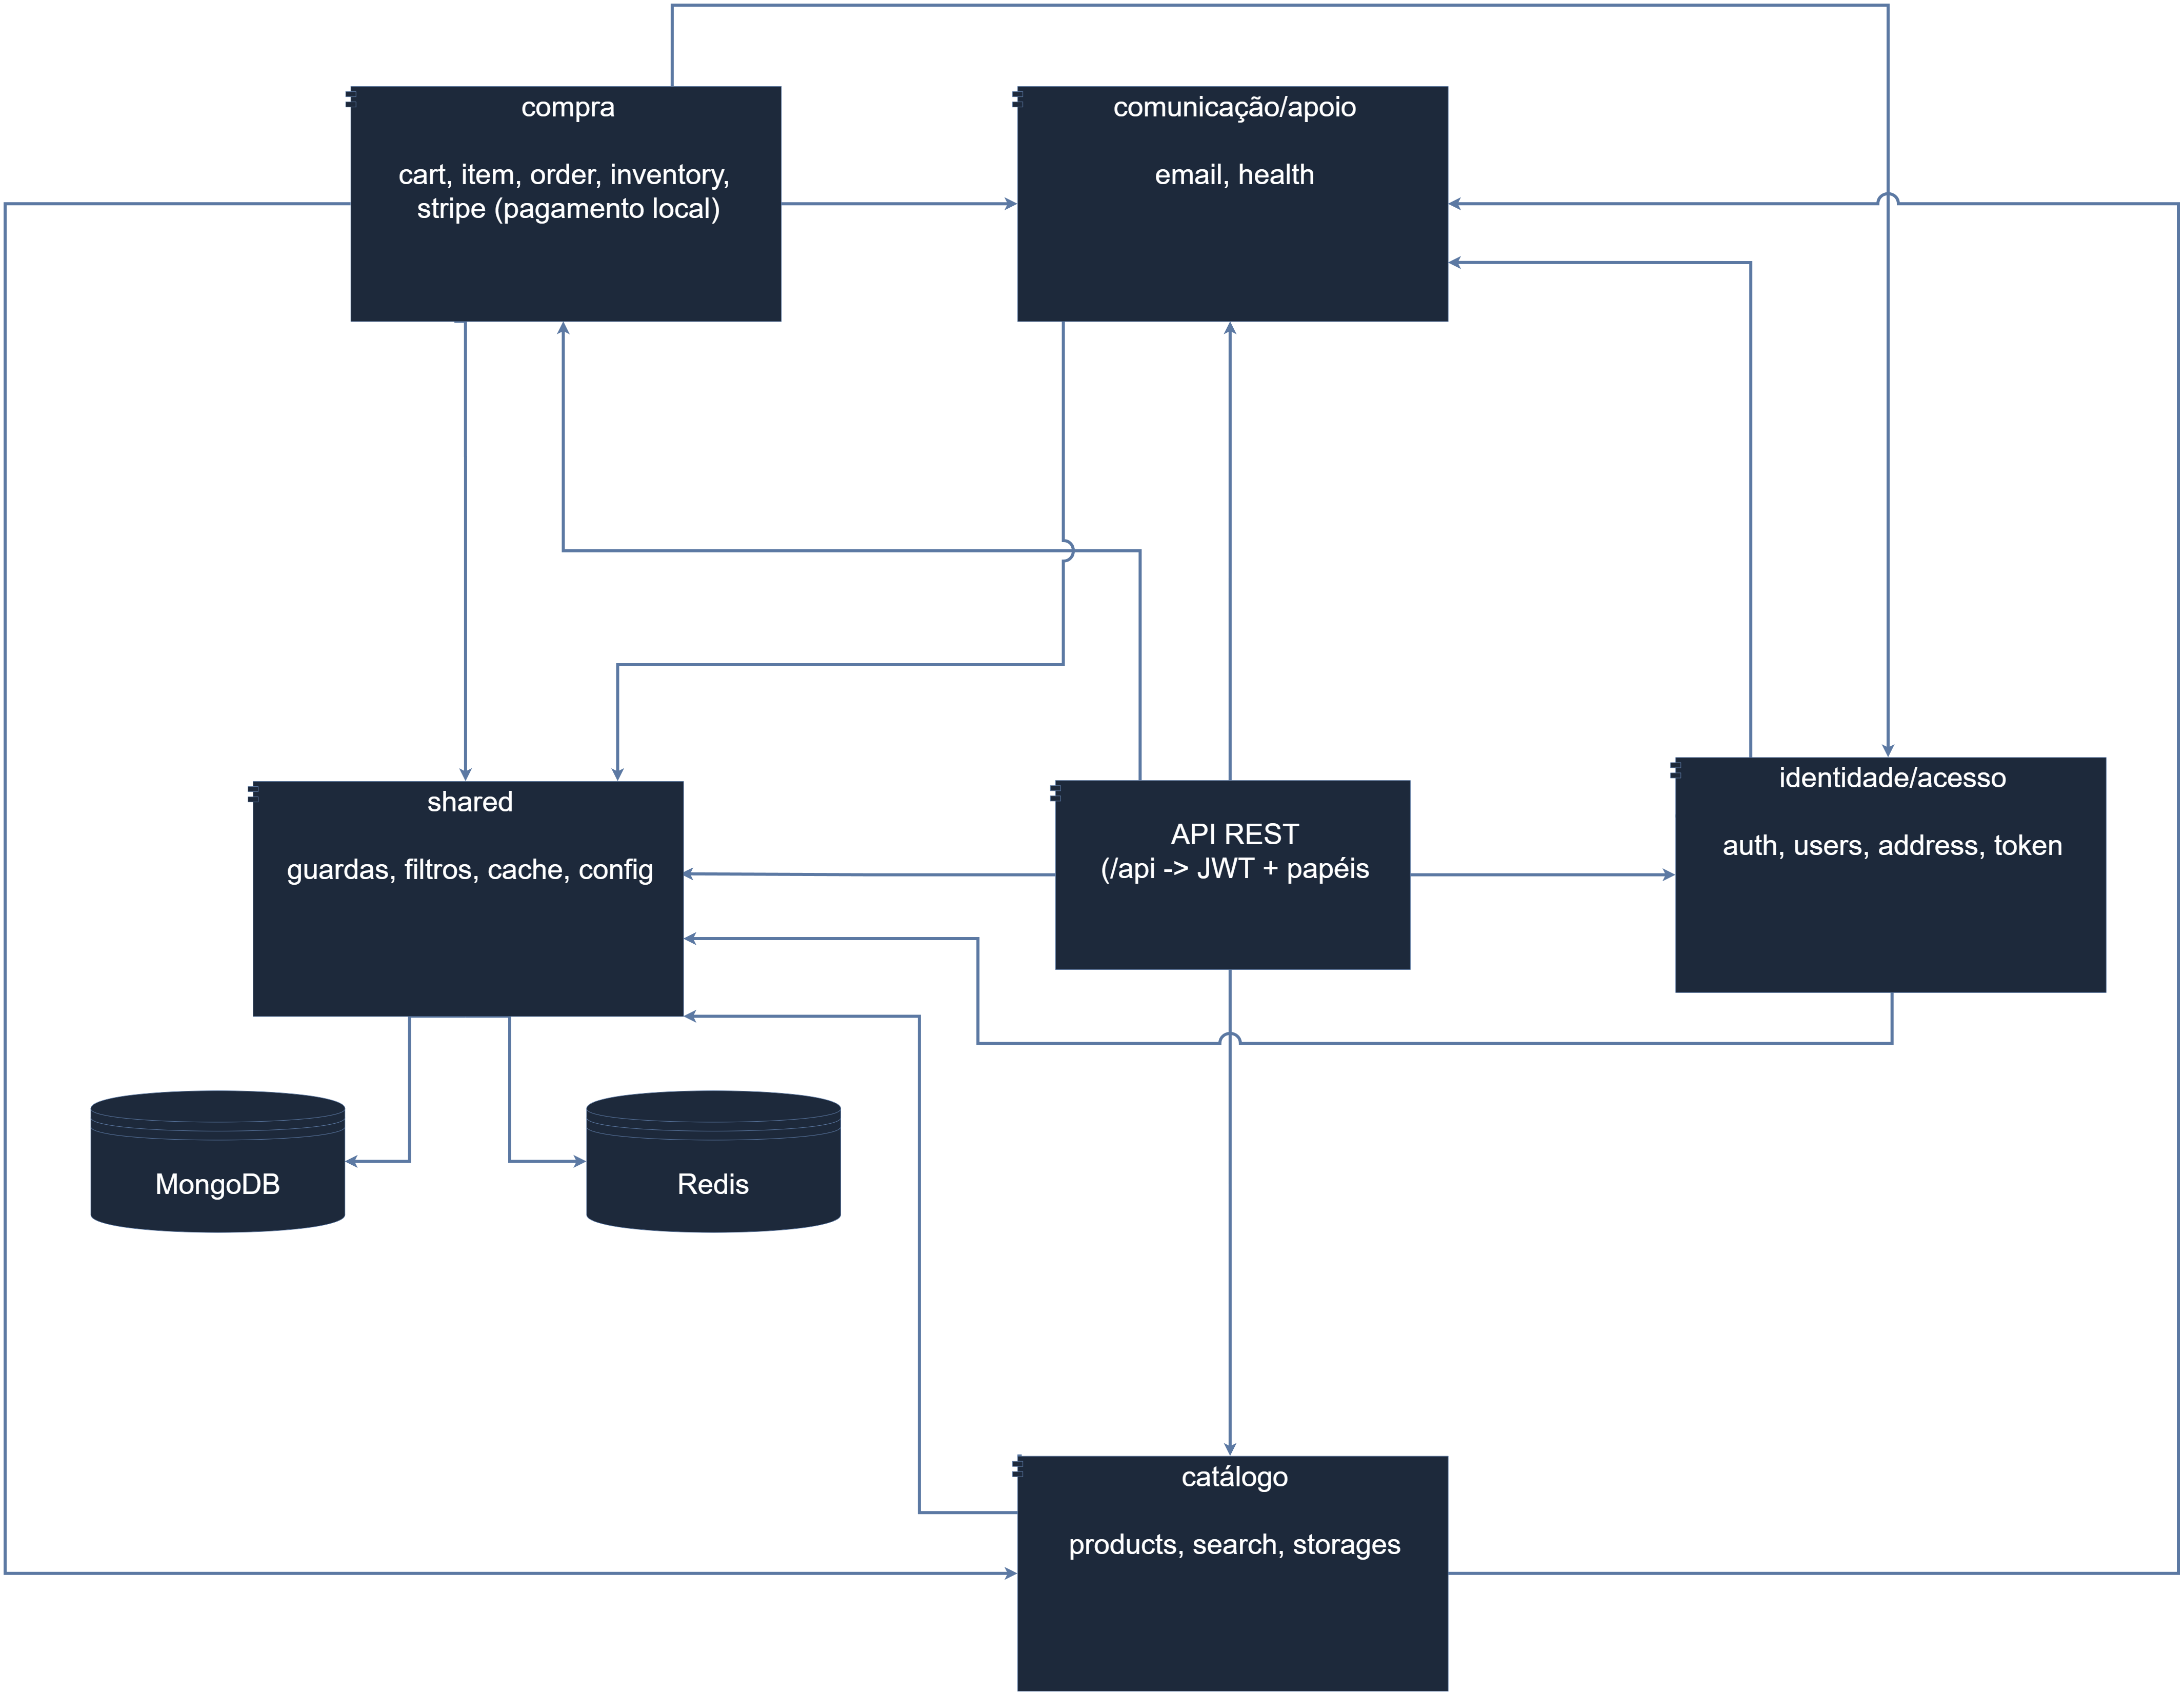
\includegraphics[width=\linewidth]{figuras/ecommerce_arquitetura.png}
    \caption{Arquitetura base do sistema de e-commerce.}
    \label{fig:ecommerce_arquitetura}
    \legend{Elaborado pelo autor (2026).}
\end{figure}

\section{Infraestrutura de Experimentação e Coleta de Métricas}
\label{sec:infra_experimental}

Para comparar as metodologias de forma precisa, é necessário configurar o ambiente para que os testes sejam feitos em cima das mesmas condições. Nesse sentido, antes de comparar as métricas, foi construída uma infraestrutura de automação, responsável por subir os sistemas, gerar a carga e coletar as métricas. Essa infraestrutura concentra os procedimentos de execução e de coleta em um único conjunto de scripts, de modo que para realizar um novo teste, não é necessário refazer manualmente o processo.

Com base nisso, as medições foram realizadas em um ambiente padrão: Windows 11, processador AMD Ryzen 7 5700X3D, 32 GB de memória, Docker Engine 29.7.2 e Docker Compose v5.4.0. Manter o ambiente permite comparar tempos de construção e consumo de recursos entre snapshots. Também, foram adotadas regras de isolamento, como manter os recursos alocados ao Docker constantes e encerrar contêineres externos ao experimento antes de cada medição, para não afetar os dados de processamento e de memória nem a contagem de componentes.

A execução de cada aplicação se apoia em contêineres Docker orquestrados por \texttt{docker compose}. Cada aplicação sobe com seus serviços de apoio, como banco de dados e, quando aplicável, cache e proxy reverso. Para que a referência base dos sistemas iniciais e decomposições partam do mesmo estado, um script de \emph{seed} determinístico popula o banco com um conjunto equivalente de dados de demonstração. As portas são fixadas por aplicação, conforme uma tabela de portas própria para o experimento, de modo a evitar colisões e preservar a reprodutibilidade.

A coleta cobre oito métricas, distribuídas nas quatro categorias de medição definidas no Capítulo \ref{cap:metodologia}: tempo de construção da imagem, tempo de inicialização, consumo de processamento e de memória em repouso e sob carga, tamanho das imagens, vazão máxima e percentis de latência sob carga, Linhas de Código, contagem de componentes físicos e violações de fronteiras lógicas. A carga sintética é gerada com a ferramenta \emph{autocannon}. A contagem de Linhas de Código e as violações de fronteiras lógicas vêm de análise estática.

Cada métrica é amostrada três vezes, e o conjunto de resultados brutos e processados é armazenado por aplicação, metodologia e snapshot. O Snapshot 0 canônico é medido uma única vez e reutilizado como referência comum no cálculo das variações; eventuais remedições de baseline ficam registradas nos dados brutos, mas não alteram a referência. As tabelas e figuras apresentadas neste capítulo são geradas automaticamente a partir desses arquivos, o que mantém a rastreabilidade entre a medição e os valores apresentados.


\section{Decomposição por Capacidade de Negócio}
\label{sec:metodologia_capacidade}

\subsection*{Sistema de Inventário}

Sob a decomposição por capacidade de negócio, os seis módulos foram agrupados pelo que a organização faz de fato. Nesse sentido, o agrupamento resultou em três capacidades, sendo elas a capacidade de Administração/Identidade, Controle de Estoque e Relatórios. A capacidade de Relatórios foi a primeira a ser extraída, por concentrar apenas consultas de leitura e não possuir dependências de entrada, ou seja, nenhum outro módulo a importa. No monólito referência, a análise estática registrou 69 dependências cruzando fronteiras de módulo, de um total de 389, sendo a maior parte delas apontando para o núcleo compartilhado.

A extração seguiu o padrão \textit{Strangler Fig} mediado por NGINX, com roteamento por prefixo de caminho: as requisições para \texttt{/api/reports/} passaram a ser encaminhadas ao novo serviço e as demais permaneceram no monólito. Adotou-se o banco de leitura compartilhado, com o serviço apontando para o mesmo PostgreSQL apenas para leitura. Como dificuldade, o módulo de relatórios dependia do mapeamento de tipos de movimentação (\texttt{MovementTypeMapper}), isto é, o único cruzamento entre domínios no monólito, e foi resolvido por uma cópia local do mapeamento, funcionando como camada anticorrupção.

A segunda capacidade extraída foi a de Administração/Identidade, que reúne a autenticação e o cadastro de usuários. Essa capacidade é pré-requisito de todos os módulos, pois cada controlador depende dos guardas de autenticação. Para extraí-la sem interromper o restante, o serviço de Identidade passou a responder por \texttt{/api/auth} e \texttt{/api/users}, enquanto o monólito manteve apenas uma cópia local dos guardas de token. Como a validação do token é feita de forma isolada, o monólito não precisa consultar a Identidade a cada requisição. Nessa fase, a persistência ainda era compartilhada entre os serviços.

A terceira e última extração foi a da capacidade de Controle de Estoque, que agrupa armazéns, produtos e movimentações, e o monólito foi desativado. Nessa etapa adotou-se a persistência isolada prevista na metodologia: a Identidade e o Estoque passaram a ter bancos próprios, e o serviço de Relatórios deixou de ter banco. Como os serviços já não compartilham tabelas, os acessos cruzados passaram a ocorrer por chamadas HTTP. A Identidade valida o armazém no Estoque ao cadastrar um usuário, e o Estoque valida o usuário na Identidade ao registrar uma movimentação, guardando o e-mail do usuário junto ao movimento. Essa separação evidenciou acoplamentos de dados que o banco compartilhado mantinha ocultos e foi a principal dificuldade da trilha. O serviço de Relatórios, por sua vez, consulta os dados do Estoque e os agrega em memória.

O Quadro \ref{qua:comp_inventory-api_capacidade-negocio_snapshots} apresenta as métricas ao longo das quatro fases e o Quadro \ref{qua:comp_capacidade-negocio_variacoes} consolida a variação acumulada da metodologia. O tempo de construção subiu de cerca de 47 segundos no baseline canônico para 138 segundos no estado final, como consequência da construção de imagens independentes. O consumo de memória e de processamento cresceu de forma contínua, com aumento significativo do processamento sob carga na fase final, quando passaram a existir dois bancos dedicados. A vazão média das rotas caiu após a primeira extração, em razão do salto adicional pelo proxy, e se recuperou nas fases seguintes. O número de componentes subiu de dois para seis. As Linhas de Código cresceram até a segunda extração, por duplicação de código transversal, e caíram no estado final, quando o monólito deixou de compor a solução. As chamadas entre fronteiras medidas pela análise estática variaram pouco, pois o acoplamento entre serviços passou a ocorrer pela rede e não é capturado por essa análise.

%% Gerado automaticamente por harness/analise/comparar.ts
\begin{quadro}[htb]
  \centering
  \caption{Inventário --- métricas por snapshot --- Capacidade de Negócio.}
  \label{qua:comp_inventory-api_capacidade-negocio_snapshots}
  \renewcommand{\arraystretch}{1.15}
  \begin{tabularx}{\textwidth}{|>{\raggedright\arraybackslash}X|r|r|r|r|}
    \hline
    \textbf{Métrica} & \textbf{S0} & \textbf{S1} & \textbf{S2} & \textbf{Final} \\ \hline
    \multicolumn{5}{|l|}{\textbf{Agilidade}} \\ \hline
    Tempo de construção (ms) & 46.746 & 116.353 & 108.405 & 138.371 \\
    Tempo de inicialização (ms) & 9.155 & 10.594 & 13.166 & 12.051 \\ \hline
    \multicolumn{5}{|l|}{\textbf{Custo}} \\ \hline
    CPU total (repouso / carga, \%) & 2,22 / 241 & 2,78 / 242,65 & 6,24 / 255,44 & 6,6 / 405,78 \\
    RAM total (repouso / carga, MB) & 86,28 / 188,47 & 149,36 / 306,32 & 186,85 / 352,72 & 203,6 / 445,1 \\
    Imagens da aplicação (MB) & 151,6 & 363,3 & 551,1 & 586,2 \\
    Componentes / contêineres & 2 / 2 & 4 / 4 & 5 / 5 & 6 / 6 \\ \hline
    \multicolumn{5}{|l|}{\textbf{Desempenho}} \\ \hline
    Vazão (média das rotas, req/s) & 355,3 & 227,4 & 266,3 & 360,1 \\
    Latência p50 (média das rotas, ms) & 62,6 & 92,7 & 77,9 & 55,2 \\ \hline
    \multicolumn{5}{|l|}{\textbf{Manutenibilidade}} \\ \hline
    Linhas de Código & 8.783 & 9.165 & 9.796 & 9.599 \\
    Chamadas entre fronteiras & 69 de 389 & 73 de 402 & 78 de 414 & 78 de 416 \\ \hline
  \end{tabularx}
  \fonte{medição automatizada do experimento (média de três execuções).}
\end{quadro}


%% Gerado automaticamente por harness/analise/comparar.ts
\begin{quadro}[htb]
  \centering
  \caption{Variação acumulada por aplicação --- Capacidade de Negócio.}
  \label{qua:comp_capacidade-negocio_variacoes}
  \renewcommand{\arraystretch}{1.15}
  \begin{tabular}{|l|r|r|r|}
    \hline
    \textbf{Métrica} & \textbf{E-commerce} & \textbf{Inventário} & \textbf{Média} \\
    \hline
    \multicolumn{4}{|l|}{\textbf{Agilidade}} \\
    \hline
    Tempo de construção (ms) & +4 \% & +196 \% & +100 \% \\
    Tempo de inicialização (ms) & +7 \% & +32 \% & +20 \% \\
    \hline
    \multicolumn{4}{|l|}{\textbf{Custo}} \\
    \hline
    CPU total (repouso / carga, \%) & $-$ 0,31 p.p. / +32 \% & +4,38 p.p. / +68 \% & +2,04 p.p. / +50 \% \\
    RAM total (repouso / carga, MB) & +46 \% / +18 \% & +136 \% / +136 \% & +91 \% / +77 \% \\
    Imagens da aplicação (MB) & +205 \% & +287 \% & +246 \% \\
    Componentes / contêineres & +3 & +4 & +4 \\
    \hline
    \multicolumn{4}{|l|}{\textbf{Desempenho}} \\
    \hline
    Vazão (média das rotas, req/s) & $-$ 1 \% & +1 \% & +0 \% \\
    Latência p50 (média das rotas, ms) & $-$ 6 \% & $-$ 12 \% & $-$ 9 \% \\
    \hline
    \multicolumn{4}{|l|}{\textbf{Manutenibilidade}} \\
    \hline
    Linhas de Código & +13 \% & +9 \% & +11 \% \\
    Chamadas entre fronteiras & $-$ 6 \% & +13 \% & +3 \% \\
    \hline
  \end{tabular}
  \fonte{medição automatizada do experimento (média de três execuções).}
\end{quadro}


\subsection*{Sistema de Leilões}


\subsection*{E-commerce}

Na decomposição por capacidade de negócio, os treze módulos do e-commerce foram agrupados em quatro capacidades: Catálogo, Clientes, Vendas e Comunicação. O planejamento inicial previa o estoque como uma capacidade à parte, mas, como ele é atualizado dentro do próprio processo de compra, foi incorporado a Vendas, junto ao carrinho e ao pedido. No monólito de referência, a análise estática identificou 79 dependências cruzando fronteiras de módulo, de um total de 207, concentradas principalmente no carrinho e no pedido.

O Catálogo foi a primeira capacidade extraída, por concentrar operações de consulta e ter poucos pontos de contato com o restante do sistema. Assim como nas demais trilhas, a extração seguiu o padrão \textit{Strangler Fig} mediado por NGINX, com a persistência ainda compartilhada. A principal consequência desta etapa foi a separação entre o pedido e a baixa de estoque, que passou a ocorrer por meio de uma chamada entre serviços. O comportamento do sistema foi preservado, mas as duas operações deixaram de ser atômicas, custo que a trilha de Transações examina de forma explícita.

Em seguida, foi extraída a capacidade de Clientes, responsável pela identidade dos usuários e da qual praticamente todos os módulos dependem. Para evitar que cada requisição precisasse consultar o novo serviço, a validação de acesso permaneceu local no monólito, e a persistência continuou compartilhada nesta fase.

Na etapa final, Vendas e Comunicação foram extraídas, o monólito foi desativado e cada serviço passou a ter seu próprio banco de dados. Com o isolamento dos dados, operações que antes eram resolvidas por consultas locais passaram a depender da rede: fechar um pedido exige validar o comprador em Clientes e os produtos no Catálogo, e exibir o carrinho requer combinar dados de dois serviços a cada leitura. Esta foi a principal dificuldade da trilha, pois o acoplamento entre as capacidades não deixou de existir, apenas foi transferido para a rede, onde a análise estática não consegue detectá-lo.

O Quadro \ref{qua:comp_ecommerce_capacidade-negocio_snapshots} apresenta as métricas das quatro fases. O tempo de construção caiu 25 \% no estado final, já que a imagem do monólito, a mais pesada, deixou de ser construída e as imagens menores passaram a ser geradas em paralelo. A inicialização variou pouco, enquanto o número de componentes subiu de três para nove com a inclusão de três bancos de dados. O impacto mais expressivo apareceu na memória, cujo consumo em repouso quase triplicou e, sob carga, praticamente dobrou.

No desempenho, a vazão média caiu 3 \% e a latência mediana recuou 12 \%. A rota de escrita apresentou aumento de vazão mesmo com as validações em rede, resultado que exige nova medição antes de ser atribuído à decomposição. As Linhas de Código cresceram 11 \% até a segunda extração e recuaram no estado final, com a remoção do monólito, e as chamadas entre fronteiras ficaram ligeiramente abaixo do código original.

Em síntese, a trilha trocou um acoplamento visível por outro invisível. O volume de código diminuiu no estado final, mas concluir um pedido passou a depender de outros serviços, um custo que escapa à análise estática e se reflete nas métricas de infraestrutura.

%% Gerado automaticamente por harness/analise/comparar.ts
\begin{quadro}[htb]
  \centering
  \caption{E-commerce --- métricas por snapshot --- Capacidade de Negócio.}
  \label{qua:comp_ecommerce_capacidade-negocio_snapshots}
  \renewcommand{\arraystretch}{1.15}
  \begin{tabularx}{\textwidth}{|>{\raggedright\arraybackslash}X|r|r|r|r|}
    \hline
    \textbf{Métrica} & \textbf{S0} & \textbf{S1} & \textbf{S2} & \textbf{Final} \\
    \hline
    \multicolumn{5}{|l|}{\textbf{Agilidade}} \\
    \hline
    Tempo de construção (ms) & 117.342 & 115.512 & 121.707 & 88.234 \\
    Tempo de inicialização (ms) & 8.032 & 8.546 & 8.634 & 8.801 \\
    \hline
    \multicolumn{5}{|l|}{\textbf{Custo}} \\
    \hline
    CPU total (repouso / carga, \%) & 0,92 / 119,87 & 0,62 / 177,19 & 0,61 / 157,72 & 1,06 / 156,06 \\
    RAM total (repouso / carga, MB) & 279,16 / 457,33 & 341,41 / 474,1 & 407,3 / 540,96 & 771,32 / 907,76 \\
    Imagens da aplicação (MB) & 98,7 & 212,2 & 301,3 & 388,8 \\
    Componentes / contêineres & 3 / 3 & 5 / 5 & 6 / 6 & 9 / 9 \\
    \hline
    \multicolumn{5}{|l|}{\textbf{Desempenho}} \\
    \hline
    Vazão (média das rotas, req/s) & 2.246,7 & 2.219 & 2.235,3 & 2.185,1 \\
    Latência p50 (média das rotas, ms) & 17,9 & 18 & 16,9 & 15,8 \\
    \hline
    \multicolumn{5}{|l|}{\textbf{Manutenibilidade}} \\
    \hline
    Linhas de Código & 4.820 & 5.169 & 5.464 & 5.328 \\
    Chamadas entre fronteiras & 79 de 207 & 80 de 210 & 74 de 211 & 76 de 206 \\
    \hline
  \end{tabularx}
  \fonte{medição automatizada do experimento (média de três execuções).}
\end{quadro}



\section{Decomposição por Subdomínio (DDD)}
\label{sec:metodologia_subdominio}

\subsection*{Sistema de Inventário}

Sob a decomposição por subdomínio, os seis módulos foram classificados pelo valor estratégico que entregam ao negócio, e não pela cadeia de processos da organização. A classificação separou o núcleo do sistema, formado pelas movimentações, dos domínios de suporte, produtos e armazéns, e dos genéricos, que reúnem a identidade e os relatórios. O núcleo é o que carrega o diferencial competitivo e concentra as regras de negócio; o suporte é necessário ao funcionamento, mas não diferencia o sistema; e os genéricos poderiam ser atendidos por componentes prontos. No monólito de referência, a análise estática registrou 69 dependências cruzando fronteiras de módulo, de um total de 389, sendo a maior parte direcionada ao núcleo compartilhado.

A extração seguiu a ordem inversa à da Capacidade de Negócio. Saíram primeiro os dois domínios genéricos, Relatórios e Identidade, por serem os de menor valor estratégico e menor risco. A extração seguiu o padrão \textit{Strangler Fig} mediado por NGINX, com roteamento por prefixo de caminho, e os serviços apontavam para o mesmo PostgreSQL. Na etapa seguinte, saiu o suporte, com produtos e armazéns, de modo que o monólito passou a conter apenas o núcleo. Até essa fase, a persistência permanecia compartilhada e não havia comunicação em rede entre os serviços.

A etapa final extraiu o núcleo e isolou a persistência, com um banco por serviço e comunicação por chamadas HTTP. Esse arranjo revelou a principal dificuldade da trilha: a regra de estoque exige, ao registrar uma movimentação, a checagem do produto e do armazém, que na decomposição por subdomínio passaram a pertencer ao serviço de suporte. Como o núcleo ficou separado do suporte, registrar uma movimentação passou a depender de validações remotas: o produto e o armazém no Suporte e o usuário na Identidade. Esse é o contraste direto com a Capacidade de Negócio, que mantinha movimentações, produtos e armazéns agrupados e preservava a verificação dentro de um único processo.

O Quadro \ref{qua:comp_inventory-api_subdominio_snapshots} apresenta as métricas ao longo das quatro fases e o Quadro \ref{qua:comp_subdominio_variacoes} consolida a variação acumulada da metodologia em relação ao S0 canônico. O tempo de construção subiu de cerca de 47 segundos no baseline para cerca de 123 segundos no estado final, em razão da construção de imagens independentes. O tempo de inicialização variou pouco até a segunda extração e subiu no estado final, quando passaram a existir três bancos. O número de componentes cresceu de dois para oito. As Linhas de Código subiram até a extração do suporte, por duplicação de código transversal, e caíram no estado final, quando o monólito deixou de compor a solução. As chamadas entre fronteiras medidas pela análise estática variaram pouco, pois o acoplamento entre serviços passou a ocorrer pela rede e não é capturado por essa análise. A vazão média das rotas apresentou leve recuperação no estado final e a latência média caiu em relação ao baseline. Vale registrar que a primeira extração desta trilha coincide, em topologia e em números, com a segunda fase da Capacidade de Negócio, o que reforça que o efeito medido até ali decorre da estrutura resultante e não da metodologia empregada.

%% Gerado automaticamente por harness/analise/comparar.ts
\begin{quadro}[htb]
  \centering
  \caption{Inventário --- métricas por snapshot --- Subdomínio (DDD).}
  \label{qua:comp_inventory-api_subdominio_snapshots}
  \renewcommand{\arraystretch}{1.15}
  \begin{tabularx}{\textwidth}{|>{\raggedright\arraybackslash}X|r|r|r|r|}
    \hline
    \textbf{Métrica} & \textbf{S0} & \textbf{S1} & \textbf{S2} & \textbf{Final} \\
    \hline
    \multicolumn{5}{|l|}{\textbf{Agilidade}} \\
    \hline
    Tempo de construção (ms) & 46.746 & 108.628 & 103.700 & 122.958 \\
    Tempo de inicialização (ms) & 9.155 & 10.056 & 9.626 & 12.540 \\
    \hline
    \multicolumn{5}{|l|}{\textbf{Custo}} \\
    \hline
    CPU total (repouso / carga, \%) & 2,22 / 241 & 4,03 / 249,96 & 2,78 / 251,4 & 2,52 / 370,73 \\
    RAM total (repouso / carga, MB) & 86,28 / 188,47 & 184,79 / 333,04 & 224,2 / 318,21 & 268,4 / 538,18 \\
    Imagens da aplicação (MB) & 151,6 & 551,2 & 737,8 & 772,9 \\
    Componentes / contêineres & 2 / 2 & 5 / 5 & 6 / 6 & 8 / 8 \\
    \hline
    \multicolumn{5}{|l|}{\textbf{Desempenho}} \\
    \hline
    Vazão (média das rotas, req/s) & 355,3 & 319,7 & 304 & 415,9 \\
    Latência p50 (média das rotas, ms) & 62,6 & 70,4 & 70,1 & 47,4 \\
    \hline
    \multicolumn{5}{|l|}{\textbf{Manutenibilidade}} \\
    \hline
    Linhas de Código & 8.783 & 9.796 & 10.310 & 10.079 \\
    Chamadas entre fronteiras & 69 de 389 & 78 de 414 & 85 de 429 & 85 de 431 \\
    \hline
  \end{tabularx}
  \fonte{medição automatizada do experimento (média de três execuções).}
\end{quadro}


%% Gerado automaticamente por harness/analise/comparar.ts
\begin{quadro}[htb]
  \centering
  \caption{Variação acumulada por aplicação --- Subdomínio (DDD).}
  \label{qua:comp_subdominio_variacoes}
  \renewcommand{\arraystretch}{1.15}
  \begin{tabular}{|l|r|r|r|}
    \hline
    \textbf{Métrica} & \textbf{E-commerce} & \textbf{Inventário} & \textbf{Média} \\
    \hline
    \multicolumn{4}{|l|}{\textbf{Agilidade}} \\
    \hline
    Tempo de construção (ms) & $-$ 37 \% & +163 \% & +63 \% \\
    Tempo de inicialização (ms) & +17 \% & +37 \% & +27 \% \\
    \hline
    \multicolumn{4}{|l|}{\textbf{Custo}} \\
    \hline
    CPU total (repouso / carga, \%) & +0,25 p.p. / +30 \% & +0,3 p.p. / +54 \% & +0,28 p.p. / +42 \% \\
    RAM total (repouso / carga, MB) & +177 \% / +98 \% & +211 \% / +186 \% & +194 \% / +142 \% \\
    Imagens da aplicação (MB) & +294 \% & +410 \% & +352 \% \\
    Componentes / contêineres & +6 & +6 & +6 \\
    \hline
    \multicolumn{4}{|l|}{\textbf{Desempenho}} \\
    \hline
    Vazão (média das rotas, req/s) & $-$ 5 \% & +17 \% & +6 \% \\
    Latência p50 (média das rotas, ms) & $-$ 7 \% & $-$ 24 \% & $-$ 16 \% \\
    \hline
    \multicolumn{4}{|l|}{\textbf{Manutenibilidade}} \\
    \hline
    Linhas de Código & +11 \% & +15 \% & +13 \% \\
    Chamadas entre fronteiras & $-$ 4 \% & +23 \% & +10 \% \\
    \hline
  \end{tabular}
  \fonte{medição automatizada do experimento (média de três execuções).}
\end{quadro}


\subsection*{Sistema de Leilões}


\subsection*{E-commerce}

Para classificar o e-commerce de acordo com seus subdomínios, o critério deixou de ser os processos que a loja executa e passou a ser o valor estratégico de cada parte do sistema. Assim, autenticação, cadastro de usuários e o envio de e-mails formam subdomínios genéricos por serem funcionalidades que podem ser terceirizadas por outros aplicativos. O catálogo de produtos é um subdomínio de suporte, pois sem ele não há venda, mas não é o que diferencia a loja. O núcleo é a parte principal do negócio, e por isso reúne carrinho, frete, pedido, estoque e pagamento.

Dois casos exigiram atenção ao código. O armazenamento de arquivos, usado tanto pelo catálogo quanto pelo cadastro de usuários, foi duplicado nos dois serviços para evitar uma dependência comum entre fronteiras. Já o pagamento, que dependia de uma plataforma externa, permaneceu no núcleo, por estar ligado à finalização do pedido e à baixa de estoque.

Assim como nos outros sistemas do experimento a ordem foi inversa à Capacidade de Negócio, começando pelos subdomínios genéricos. Na primeira fase, Identidade e Comunicação foram extraídas, ainda com o banco de dados compartilhado. A principal dificuldade foi desfazer dependências circulares entre usuários e autenticação, que se referenciavam um ao outro no monólito. Como nas outras trilhas, a validação de acesso permaneceu local, evitando consultas à Identidade a cada requisição. Essa fase reduziu as dependências entre fronteiras de 79 para 69, já que o monólito ainda concentrava o catálogo e o próprio serviço de Identidade recriou parte dessas dependências internamente.

O Catálogo foi extraído em seguida, por ser o último componente que o monólito ainda acessava diretamente no banco. Nesta fase, apenas a baixa de estoque passou a ser feita por chamada ao novo serviço, enquanto carrinho e pedido continuaram lendo os produtos no banco compartilhado. Com isso, a confirmação do pedido e a baixa de estoque deixaram de ocorrer na mesma transação, e uma falha entre as duas pode deixar o sistema inconsistente. Por outro lado, as consultas ao catálogo ganharam de 4 \% a 6 \% de vazão com o processo dedicado.

Na etapa final, o núcleo foi extraído, o monólito foi desativado e cada serviço passou a ter seu próprio banco de dados. A partir daí, o custo deixou de estar no código e passou a estar na rede, visto que para fechar um pedido é necessário validar o comprador na Identidade e os produtos no Catálogo, e exibir o carrinho requer combinar dados de dois serviços a cada leitura. Manter pagamento, pedido e estoque juntos evitou uma transação distribuída, mas não eliminou essas consultas cruzadas. Mais uma vez, o acoplamento não desapareceu, apenas saiu do alcance da análise estática.

O Quadro \ref{qua:comp_ecommerce_subdominio_snapshots} mostra dois efeitos distintos. O primeiro é o custo de manter mais processos em execução, já que com nove contêineres no lugar de três, o consumo de memória quase triplicou em repouso e praticamente dobrou sob carga. O segundo só aparece no estado final, quando o monólito deixa de ser construído. Nesse cenário, o tempo de build caiu 37 \% em relação ao baseline, depois de subir levemente nas fases intermediárias, e as Linhas de Código recuaram em relação ao pico atingido durante a migração. O desempenho variou pouco ao longo da trilha. A vazão média caiu na primeira fase, aumentou em seguida e terminou cerca de 5 \% abaixo do baseline, enquanto a latência mediana ficou 7 \% menor.

% Gerado automaticamente por harness/analise/comparar.ts
\begin{quadro}[htb]
  \centering
  \caption{E-commerce --- métricas por snapshot --- Subdomínio (DDD).}
  \label{qua:comp_ecommerce_subdominio_snapshots}
  \renewcommand{\arraystretch}{1.15}
  \begin{tabularx}{\textwidth}{|>{\raggedright\arraybackslash}X|r|r|r|r|}
    \hline
    \textbf{Métrica} & \textbf{S0} & \textbf{S1} & \textbf{S2} & \textbf{Final} \\
    \hline
    \multicolumn{5}{|l|}{\textbf{Agilidade}} \\
    \hline
    Tempo de construção (ms) & 117.342 & 123.877 & 126.788 & 73.856 \\
    Tempo de inicialização (ms) & 8.032 & 8.976 & 9.292 & 9.420 \\
    \hline
    \multicolumn{5}{|l|}{\textbf{Custo}} \\
    \hline
    CPU total (repouso / carga, \%) & 0,92 / 119,87 & 1,05 / 153,1 & 1,15 / 155,91 & 1,17 / 155,66 \\
    RAM total (repouso / carga, MB) & 279,16 / 457,33 & 376,43 / 517,4 & 436,9 / 573,15 & 773,82 / 904,8 \\
    Imagens da aplicação (MB) & 98,7 & 310,1 & 398,5 & 388,8 \\
    Componentes / contêineres & 3 / 3 & 6 / 6 & 7 / 7 & 9 / 9 \\
    \hline
    \multicolumn{5}{|l|}{\textbf{Desempenho}} \\
    \hline
    Vazão (média das rotas, req/s) & 2.246,7 & 2.025,4 & 2.118,9 & 2.139,5 \\
    Latência p50 (média das rotas, ms) & 17,9 & 17,2 & 17,3 & 16,7 \\
    \hline
    \multicolumn{5}{|l|}{\textbf{Manutenibilidade}} \\
    \hline
    Linhas de Código & 4.820 & 5.346 & 5.614 & 5.328 \\
    Chamadas entre fronteiras & 79 de 207 & 69 de 209 & 69 de 210 & 76 de 206 \\
    \hline
  \end{tabularx}
  \fonte{medição automatizada do experimento (média de três execuções).}
\end{quadro}


Ao final, a trilha chegou às mesmas quatro fronteiras da Capacidade de Negócio, com o mesmo volume de código e o mesmo número de chamadas entre fronteiras. Como o e-commerce é organizado em torno de um único fluxo de negócio, os critérios de valor e de processo acabam convergindo para o mesmo resultado, delimitado pelo início e pelo fim da compra. O que muda é o percurso. Começar pelos subdomínios genéricos reduziu o acoplamento estático já na primeira fase e antecipou o custo de infraestrutura, enquanto a Capacidade de Negócio só observou essa redução na segunda fase. Neste sistema, portanto, a metodologia escolhida altera o momento em que o custo é pago, e não a arquitetura obtida.



\section{Decomposição por Transações}
\label{sec:metodologia_transacoes}

\subsection*{Sistema de Inventário}

Na decomposição por transações, o agrupamento parte do que precisa ser gravado de forma individual. No sistema de inventário, a regra que impede retirar mais do que existe e o cálculo de estoque a partir das movimentações exigem que a verificação de produto e de armazém e a escrita do movimento ocorram na mesma transação. Por isso, armazéns, produtos e movimentações formaram um único serviço, o Estoque. A Identidade e os Relatórios ficaram fora dessa fronteira, sendo que a primeira fornece o usuário referenciado pelo movimento, e os segundos apenas leem os dados. No monólito de referência, a análise estática registrou 69 dependências cruzando fronteiras de módulo, de um total de 389.

A ordem de extração foi o oposto da adotada na Capacidade de Negócio: o grupo atômico saiu primeiro, para que a consistência transacional fosse preservada em um único processo desde o início. A extração seguiu o padrão \textit{Strangler Fig} mediado por NGINX, com as rotas de armazéns, produtos e movimentações desviadas para o novo serviço. Nessa fase, a persistência era compartilhada, e o Estoque passou a validar o usuário no monólito por um endpoint interno. Para manter o e-mail do usuário no histórico de movimentações, foi adicionada a coluna \texttt{user\_email} à tabela de movimentos, já que a Identidade ainda não era um serviço separado.

A segunda extração foi a da Identidade. O monólito manteve apenas os Relatórios e uma cópia local dos guardas de autenticação, que validam o token sem consultar outro serviço. O Estoque passou a validar o usuário na Identidade, e a Identidade passou a validar o armazém no Estoque, ambas por chamadas HTTP. A persistência continuou compartilhada, de modo que os Relatórios seguiam lendo os dados de estoque diretamente no banco.

Na etapa final, os Relatórios foram extraídos, o monólito foi desativado e a persistência foi isolada, com um banco para a Identidade e outro para o Estoque. O serviço de Relatórios deixou de ter banco e passou a consultar a API interna do Estoque. A principal dificuldade da trilha foi o acoplamento entre movimento e usuário: como o usuário deixou de estar no mesmo banco do movimento, sua validação passou a ser remota e o e-mail foi desnormalizado no registro da movimentação. É a mesma dificuldade observada na Capacidade de Negócio, mas aqui ela aparece desde a primeira extração.

Os Quadros \ref{qua:comp_inventory-api_transacoes_snapshots} e \ref{qua:comp_transacoes_variacoes} apresentam as métricas ao longo das fases e a variação acumulada da metodologia. O tempo de construção subiu de cerca de 47 segundos no baseline para cerca de 112 segundos no estado final, em razão da construção de imagens independentes. O tempo de inicialização subiu de cerca de 9 segundos para cerca de 14 segundos. O número de componentes cresceu de dois para seis. As Linhas de Código subiram até a segunda extração, por duplicação de código transversal, e caíram no estado final, quando o monólito deixou de compor a solução. As chamadas entre fronteiras medidas pela análise estática variaram pouco, pois o acoplamento entre serviços passou a ocorrer pela rede e não é capturado por essa análise. No estado final, a vazão média das rotas ficou cerca de 8\% acima do baseline e a latência mediana caiu cerca de 18\%.

O estado final coincide com o da Capacidade de Negócio: mesma topologia, mesmas 9.599 Linhas de Código e as mesmas 78 de 416 chamadas entre fronteiras. A diferença está na ordem das extrações. Nesta trilha, o grupo atômico saiu na primeira extração, e o caminho de escrita passou a depender da rede antes das demais metodologias; na Capacidade, a escrita permaneceu local até o estado final. O resultado indica que, neste domínio, o critério de transações converge para a mesma fronteira da capacidade, porque a invariante de estoque domina o agrupamento. A comparação relevante deixa de ser o formato final e passa a ser quando o custo é pago e por quanto tempo a consistência da escrita depende de um único processo.

%% Gerado automaticamente por harness/analise/comparar.ts
\begin{quadro}[htb]
  \centering
  \caption{Inventário --- métricas por snapshot --- Transações.}
  \label{qua:comp_inventory-api_transacoes_snapshots}
  \renewcommand{\arraystretch}{1.15}
  \begin{tabularx}{\textwidth}{|>{\raggedright\arraybackslash}X|r|r|r|r|}
    \hline
    \textbf{Métrica} & \textbf{S0} & \textbf{S1} & \textbf{S2} & \textbf{Final} \\
    \hline
    \multicolumn{5}{|l|}{\textbf{Agilidade}} \\
    \hline
    Tempo de construção (ms) & 46.746 & 75.321 & 99.791 & 111.724 \\
    Tempo de inicialização (ms) & 9.155 & 9.788 & 12.537 & 14.028 \\
    \hline
    \multicolumn{5}{|l|}{\textbf{Custo}} \\
    \hline
    CPU total (repouso / carga, \%) & 2,22 / 241 & 1,95 / 259,31 & 3,13 / 247,83 & 1,75 / 433,39 \\
    RAM total (repouso / carga, MB) & 86,28 / 188,47 & 146,86 / 305,28 & 185,32 / 327,95 & 203,03 / 421,79 \\
    Imagens da aplicação (MB) & 151,6 & 363,5 & 551,3 & 586,6 \\
    Componentes / contêineres & 2 / 2 & 4 / 4 & 5 / 5 & 6 / 6 \\
    \hline
    \multicolumn{5}{|l|}{\textbf{Desempenho}} \\
    \hline
    Vazão (média das rotas, req/s) & 355,3 & 329,5 & 314 & 384,2 \\
    Latência p50 (média das rotas, ms) & 62,6 & 64,9 & 67,8 & 51,6 \\
    \hline
    \multicolumn{5}{|l|}{\textbf{Manutenibilidade}} \\
    \hline
    Linhas de Código & 8.783 & 9.431 & 9.856 & 9.599 \\
    Chamadas entre fronteiras & 69 de 389 & 77 de 408 & 81 de 419 & 78 de 416 \\
    \hline
  \end{tabularx}
  \fonte{medição automatizada do experimento (média de três execuções).}
\end{quadro}


%% Gerado automaticamente por harness/analise/comparar.ts
\begin{quadro}[htb]
  \centering
  \caption{Variação acumulada por aplicação --- Transações.}
  \label{qua:comp_transacoes_variacoes}
  \renewcommand{\arraystretch}{1.15}
  \begin{tabular}{|l|r|r|r|}
    \hline
    \textbf{Métrica} & \textbf{E-commerce} & \textbf{Inventário} & \textbf{Média} \\
    \hline
    \multicolumn{4}{|l|}{\textbf{Agilidade}} \\
    \hline
    Tempo de construção (ms) & $-$ 28 \% & +139 \% & +56 \% \\
    Tempo de inicialização (ms) & +4 \% & +53 \% & +29 \% \\
    \hline
    \multicolumn{4}{|l|}{\textbf{Custo}} \\
    \hline
    CPU total (repouso / carga, \%) & +0,31 p.p. / +32 \% & $-$ 0,47 p.p. / +80 \% & $-$ 0,08 p.p. / +56 \% \\
    RAM total (repouso / carga, MB) & +174 \% / +97 \% & +135 \% / +124 \% & +155 \% / +110 \% \\
    Imagens da aplicação (MB) & +294 \% & +287 \% & +291 \% \\
    Componentes / contêineres & +6 & +4 & +5 \\
    \hline
    \multicolumn{4}{|l|}{\textbf{Desempenho}} \\
    \hline
    Vazão (média das rotas, req/s) & $-$ 3 \% & +8 \% & +3 \% \\
    Latência p50 (média das rotas, ms) & $-$ 6 \% & $-$ 18 \% & $-$ 12 \% \\
    \hline
    \multicolumn{4}{|l|}{\textbf{Manutenibilidade}} \\
    \hline
    Linhas de Código & +4 \% & +9 \% & +7 \% \\
    Chamadas entre fronteiras & $-$ 10 \% & +13 \% & +1 \% \\
    \hline
  \end{tabular}
  \fonte{medição automatizada do experimento (média de três execuções).}
\end{quadro}


\subsection*{Sistema de Leilões}

\subsection*{E-commerce}

Na decomposição por transações, o agrupamento parte do que precisa ser gravado junto. No e-commerce, a operação crítica é a confirmação do pedido: o webhook de pagamento muda o status do pedido e baixa o estoque dos itens na mesma sessão Mongo. Se as duas escritas não acontecem juntas, um pedido pode ficar pago sem baixa ou com baixa parcial. Por isso, carrinho, frete, pedido, estoque e pagamento formaram um único serviço, o Checkout. Catálogo, Identidade e Comunicação ficaram fora da transação. O código de origem tinha 79 de 207 dependências cruzando fronteiras de módulo, concentradas no carrinho e no pedido.

A extração começou pelo Checkout, ao contrário das outras duas trilhas, para que a transação ficasse em um único processo desde o início. O banco continuou sendo o do monólito: carrinho e pedido liam produtos e usuários na mesma base, e a baixa do estoque seguia dentro da sessão do pedido. O monólito perdeu cinco módulos e manteve catálogo, identidade e comunicação, além de duas rotas internas: uma para o e-mail de confirmação, chamado depois do commit, e outra para o status de assinatura.

Na segunda fase, o Catálogo foi extraído. A leitura de produto continuou local, porque a coleção era a mesma, e a baixa de estoque passou a escrever uma coleção que outro serviço serve. A atomicidade sobreviveu apenas porque o banco continuava compartilhado: a escrita cruzava a fronteira do serviço, mas não a do banco. É uma situação que só existe durante a migração e que a etapa final remove.

Na etapa final, Identidade e Comunicação saíram, o monólito foi desativado e cada serviço passou a ter seu banco. O estoque deixou de ser um campo do produto e virou um contador próprio do Checkout, baixado na mesma sessão do status do pedido. O Catálogo mantém uma cópia de leitura, atualizada por uma chamada depois do commit, e a criação de um produto inicializa o contador no Checkout. Se a sincronização falhar, a listagem mostra saldo antigo, mas o saldo que decide a venda continua consistente. A validação do comprador e do item virou chamada HTTP dentro do caminho de escrita.

O Quadro \ref{qua:comp_ecommerce_transacoes_snapshots} apresenta as métricas das quatro fases. O tempo de construção subiu de 117,3 para 129,2 segundos nas duas primeiras extrações e caiu para 84,7 segundos no estado final, 27,8 \% abaixo do baseline, porque a imagem do monólito deixou de ser construída. As Linhas de Código foram de 4.820 para 5.263 e terminaram em 5.004, com a saída do monólito. As chamadas entre fronteiras caíram de 79 para 72 e terminaram em 71 de 193. Os componentes passaram de três para nove e a memória em repouso, de 279,2 para 764,5 MB, com os três bancos. A vazão média terminou 3 \% abaixo do baseline e a latência mediana, 5,6 \% menor.

A rota de escrita medida nas outras trilhas não executa essa transação: \texttt{POST /api/orders} apenas grava o pedido. Por isso, esta trilha mediu também o webhook, com uma conexão, porque requisições concorrentes sobre o mesmo pedido disputam a mesma transação e falham com conflito de escrita. O webhook fez 75,6 req/s no s1, 91,2 no s2 e 77,1 no final; a queda de 15,5 \% no último passo corresponde às duas validações em rede e à sincronização da cópia de leitura.

% Gerado automaticamente por harness/analise/comparar.ts
\begin{quadro}[htb]
  \centering
  \caption{E-commerce --- métricas por snapshot --- Transações.}
  \label{qua:comp_ecommerce_transacoes_snapshots}
  \renewcommand{\arraystretch}{1.15}
  \begin{tabularx}{\textwidth}{|>{\raggedright\arraybackslash}X|r|r|r|r|}
    \hline
    \textbf{Métrica} & \textbf{S0} & \textbf{S1} & \textbf{S2} & \textbf{Final} \\
    \hline
    \multicolumn{5}{|l|}{\textbf{Agilidade}} \\
    \hline
    Tempo de construção (ms) & 117.342 & 120.345 & 129.214 & 84.658 \\
    Tempo de inicialização (ms) & 8.032 & 8.578 & 8.659 & 8.366 \\
    \hline
    \multicolumn{5}{|l|}{\textbf{Custo}} \\
    \hline
    CPU total (repouso / carga, \%) & 0,92 / 119,87 & 0,97 / 151,7 & 0,93 / 156,46 & 1,23 / 157,96 \\
    RAM total (repouso / carga, MB) & 279,16 / 457,33 & 358,69 / 537,47 & 406,31 / 537,68 & 764,52 / 901,1 \\
    Imagens da aplicação (MB) & 98,7 & 212,7 & 301,2 & 388,8 \\
    Componentes / contêineres & 3 / 3 & 5 / 5 & 6 / 6 & 9 / 9 \\
    \hline
    \multicolumn{5}{|l|}{\textbf{Desempenho}} \\
    \hline
    Vazão (média das rotas, req/s) & 2.246,7 & 2.024,6 & 2.091,5 & 2.179,8 \\
    Latência p50 (média das rotas, ms) & 17,9 & 17,3 & 17,1 & 16,9 \\
    \hline
    \multicolumn{5}{|l|}{\textbf{Manutenibilidade}} \\
    \hline
    Linhas de Código & 4.820 & 4.938 & 5.263 & 5.004 \\
    Chamadas entre fronteiras & 79 de 207 & 72 de 196 & 71 de 197 & 71 de 193 \\
    \hline
  \end{tabularx}
  \fonte{medição automatizada do experimento (média de três execuções).}
\end{quadro}


O estado final tem as mesmas quatro fronteiras das outras duas trilhas, mas não o mesmo artefato: 5.004 Linhas de Código e 71 de 193 chamadas, contra 5.328 e 76 de 206. A diferença não é de forma: o estoque está dentro do Checkout. Na Capacidade e no Subdomínio, a baixa saía por chamada HTTP e o pedido deixava de ser atômico desde a primeira extração; aqui, a consistência foi preservada em todas as fases, ao preço de extrair cinco módulos de uma vez, de quase dobrar a memória e de reduzir a vazão do caminho de confirmação. Em um domínio com um único fluxo de negócio, o critério de transações chega à mesma topologia dos outros dois, mas o custo é pago no começo, e não no fim.

\section{Comparação entre as Metodologias}
\label{sec:comparacao_metodologias}

O Quadro \ref{qua:comp_metodologias} reúne a variação acumulada de cada metodologia entre o estado inicial e o estado final.


%%% Gerado automaticamente por harness/analise/comparar.ts
\begin{quadro}[htb]
  \centering
  \caption{Variação acumulada por metodologia (S0 $\rightarrow$ último snapshot).}
  \label{qua:comp_metodologias}
  \renewcommand{\arraystretch}{1.15}
  \setlength{\tabcolsep}{4pt}
  \begin{tabularx}{\textwidth}{|>{\raggedright\arraybackslash}X|r|r|r|}
    \hline
    \textbf{Métrica} & \textbf{Capacidade de Negócio} & \textbf{Subdomínio (DDD)} & \textbf{Transações} \\
    \hline
    \multicolumn{4}{|l|}{\textbf{Agilidade}} \\
    \hline
    Tempo de construção (ms) & +196 \% & +63 \% & +139 \% \\
    Tempo de inicialização (ms) & +32 \% & +27 \% & +53 \% \\
    \hline
    \multicolumn{4}{|l|}{\textbf{Custo}} \\
    \hline
    CPU total (repouso / carga, \%) & +4,38 p.p. / +68 \% & +0,28 p.p. / +42 \% & $-$ 0,47 p.p. / +80 \% \\
    RAM total (repouso / carga, MB) & +136 \% / +136 \% & +194 \% / +142 \% & +135 \% / +124 \% \\
    Imagens da aplicação (MB) & +287 \% & +352 \% & +287 \% \\
    Componentes / contêineres & +4 & +6 & +4 \\
    \hline
    \multicolumn{4}{|l|}{\textbf{Desempenho}} \\
    \hline
    Vazão (média das rotas, req/s) & +1 \% & +6 \% & +8 \% \\
    Latência p50 (média das rotas, ms) & $-$ 12 \% & $-$ 16 \% & $-$ 18 \% \\
    \hline
    \multicolumn{4}{|l|}{\textbf{Manutenibilidade}} \\
    \hline
    Linhas de Código & +9 \% & +13 \% & +9 \% \\
    Chamadas entre fronteiras & +13 \% & +10 \% & +13 \% \\
    \hline
  \end{tabularx}
  \fonte{elaborado pelo autor (2026) a partir da medição automatizada.}
\end{quadro}


\section{Síntese do Capítulo}
\label{sec:sintese_capitulo}

\chapter{Conclusão}

Este capítulo apresentará as considerações finais, a avaliação dos resultados alcançados pela metodologia proposta e as direções para trabalhos futuros.

\section{Contribuições}

\section{Limitações}

\section{Trabalhos Futuros}

% Referências (geradas automaticamente a partir do bloco 3)
\elementospostextuais

% =========================================================================
% 7. APÊNDICES E ANEXOS                                          (OPCIONAL)
%    Comente (%) a linha correspondente se não houver.
% =========================================================================
% ---
% Inicia os apêndices
% ---
\begin{apendicesenv}

% ----------------------------------------------------------
\chapter{Primeiro Apêndice}
% ----------------------------------------------------------

Apêndice é um elemento opcional do trabalho acadêmico composto por documentos ou materiais elaborados pelo próprio autor como complemento de sua argumentação, demonstração ou desenvolvimento do tema. Diferentemente dos anexos, os apêndices são produzidos pelo autor do trabalho e podem incluir questionários aplicados, roteiros de entrevista, formulários, códigos-fonte desenvolvidos, demonstrações matemáticas detalhadas, ou qualquer outro material complementar criado especificamente para subsidiar a pesquisa.

% ----------------------------------------------------------
\chapter{Segundo Apêndice}
% ----------------------------------------------------------

Conteúdo do Segundo Apêndice

\end{apendicesenv}
% ---
\begin{anexosenv}

% ----------------------------------------------------------
\chapter{Primeiro Anexo}
% ----------------------------------------------------------

Anexo é um elemento opcional do trabalho acadêmico que consiste em documentos ou materiais não elaborados pelo autor, mas que servem como complemento, fundamentação ou ilustração do conteúdo apresentado. Os anexos podem incluir legislação, normativas técnicas, mapas, fotografias, tabelas de terceiros, documentos oficiais, entre outros materiais que, embora relevantes para a compreensão do trabalho, não foram produzidos pelo próprio autor.

% ----------------------------------------------------------
\chapter{Segundo Anexo}
% ----------------------------------------------------------

Conteúdo do Segundo Anexo

\end{anexosenv}

\end{document}
